\documentclass[a4paper,12pt]{article}
\usepackage{a4wide}
\usepackage[T1]{fontenc}
\usepackage{lmodern}
\usepackage{textcomp} 
\usepackage[utf8]{inputenc}
\usepackage{xcolor}
\usepackage[czech,english]{babel}
\usepackage[pdftex, final]{graphicx}
% \usepackage[pdftex, final, colorlinks=true]{hyperref}
\usepackage{verbatim}
\usepackage{alltt}
\usepackage{paralist}
\usepackage{mdwlist}
\usepackage{subfig}
\usepackage[final]{pdfpages}
%\usepackage[hyphens]{url}
%\PassOptionsToPackage{hyphens}{url}

\usepackage[final,pdftex,colorlinks=false,breaklinks=true]{hyperref}
\usepackage[hyphenbreaks]{breakurl}

%%%%%%%%%%%%%%%%%%%%%%%%%
% pro podmineny preklad
% false je defaultně


% \newif\ifbc % Pouze do bakalářské práce
%  \bctrue

%%%%%%%%%% fancy %%%%%%%%%%%
\usepackage{fancyhdr}

\fancyhead[L]{ČVUT v~Praze}

\setlength{\headheight}{16pt}

% \usepackage{stdpage}


%%%%%%%%%%%% rozmery %%%%%%%%%%%%%%%%%%
\usepackage[%
%top=40mm,
%bottom=35mm,
%left=40mm,
%right=30mm
top=40mm,
bottom=35mm,
left=35mm,
right=25mm
]{geometry}


\renewcommand\baselinestretch{1.3}
\parskip=0.8ex plus 0.4ex minus 0.1 ex

\newcommand{\klicslova}[2]{\noindent\textbf{#1: }#2}
\newcommand{\modul}[1]{\emph{#1}}
\author{Štěpán Turek}
% \pagecolor{darkGrey}
\newcommand{\necislovana}[1]{%
\phantomsection
\addcontentsline{toc}{section}{#1}
\section*{#1}
\markboth{\uppercase{#1}}{}
}

%%%%%%%%%%%%%%%%%%%%%%%%%%%%%%
\begin{document}
\pagestyle{empty}

\begin{center}
%napisy
\newcommand{\napisCVUT}{České vysoké učení technické v Praze}
\newcommand{\napisFS}{Fakulta stavební}
\newcommand{\napisObor}{Obor geoinformatika}
\newcommand{\napisKatedra}{Katedra mapování a kartografie}
\newcommand{\napisVedouci}{Ing. Martin Landa}
\newcommand{\napisAutor}{Štěpán Turek}
\newcommand{\napisDatum}{Praha 2012}
\newcommand{\napisNazevI}{Implementace podpory WMS }
\newcommand{\napisNazevII}{do programů GRASS GIS a SAGA GIS}
\newcommand{\napisNazevAjI}{Implementation of WMS support}
\newcommand{\napisNazevAjII}{in GRASS GIS and SAGA GIS}
\newcommand{\napisBakalarka}{Bakalářská práce}
\newcommand{\napisPraha}{Praha 2012}
%
% prikazy
%\newcommand{\velka}[1]{\uppercase{#1}}
\newcommand{\velka}[1]{\textsc{#1}}
%
% 
\newif\ifpatitul
\patitultrue

\ifpatitul
{\Large\velka{\napisCVUT}}\\
\velka{\Large\napisFS}\\
\vfill
{\LARGE\velka{\napisBakalarka}}
\vfill
{\large\napisPraha\hfill\napisAutor}
\newpage
\fi%patitul


{\Large\velka{\napisCVUT}}\\
{\Large\velka{\napisFS}}\\
{\Large\velka{\napisObor}}
\vfill

\includegraphics[width=3cm]{logo_cvut_cb} %~
\vfill
{\Large\velka{\napisBakalarka}}\\
{\Large\velka{\napisNazevI\\
\napisNazevII}}\\
{\large\velka{\napisNazevAjI\\
\napisNazevAjII}}
\vfill
{\large%
Vedoucí práce: \napisVedouci\\
\napisKatedra\\
\bigskip
\napisDatum\hfill\napisAutor}
\end{center}

\newpage
\definecolor{navodotisk}{RGB}{10,10,10}
\newcommand{\vlozZadani}{%
\Huge\textcolor{navodotisk}{\textsf{\textbf{ZDE VLOŽIT ORIGINÁLNÍ ZADÁNÍ}}}%
}
%%%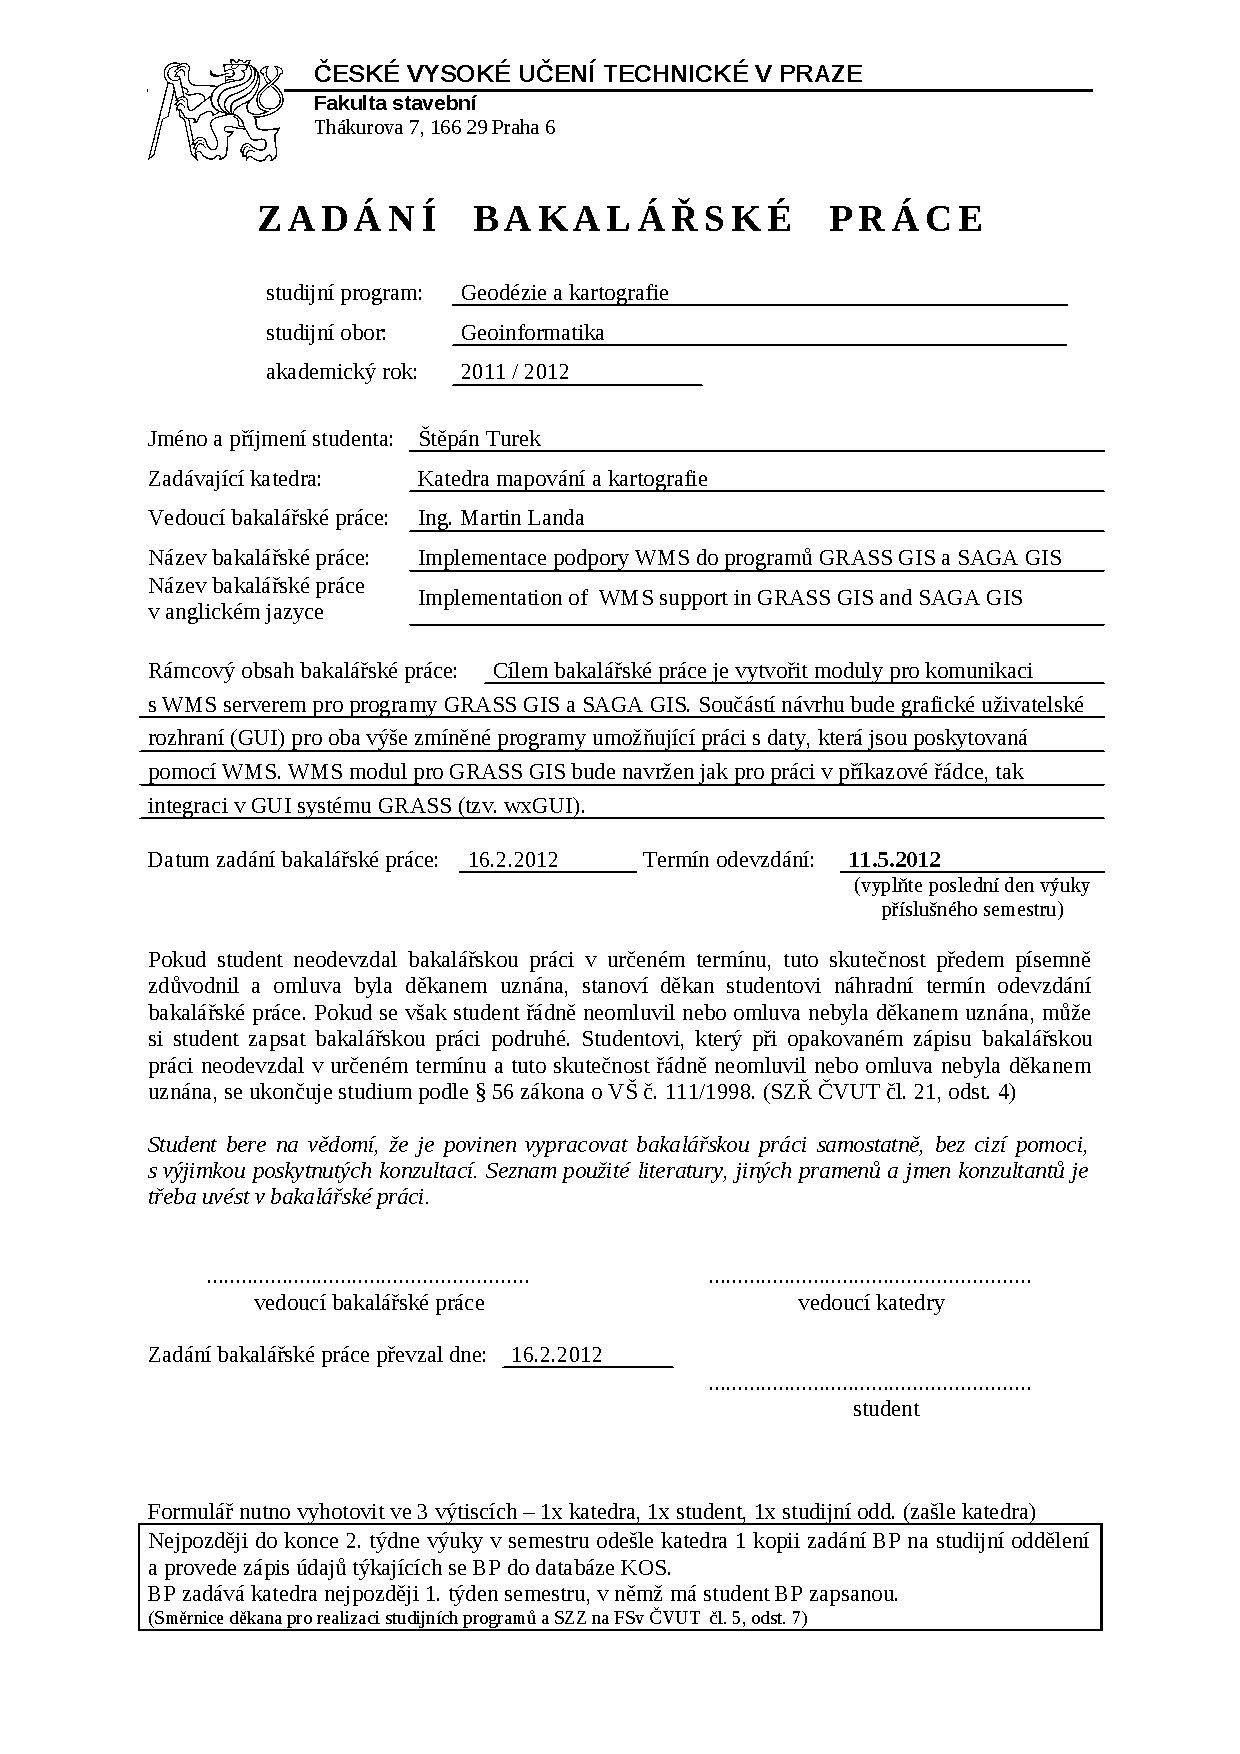
\includepdf[picturecommand={\put(100,200){\vlozZadani}}]{zadani}
 % resi si zalomeni sam





\begin{abstract}

\bigskip
Cílem této práce je zlepšit podporu WMS v~programech GRASS GIS a 
SAGA GIS. Stávající podpora je v~obou programech nedostatečná, což
je nepříjemným omezením pro uživatele. Ti přicházejí o~možnost využití řady  zdrojů rastrových dat, která jsou prostřednictvím WMS serverů poskytována.

V~úvodu práce je čtenář seznámen s~principy 
fungování WMS z~pohledu klienta, který komunikuje s~WMS serverem.

Další části práce se věnují vytvořeným WMS modulům pro GRASS GIS a SAGA GIS.
U~obou modulů je popsán průběh jejich vývoje. Také jsou uvedeny návody pro 
práci s~těmito moduly. 
\bigskip

\klicslova{Klíčová slova}{GIS, GRASS, SAGA, WMS}

\end{abstract}

\selectlanguage{english}
\begin{abstract}

The aim of the thesis is improvement of WMS support in GRASS GIS and SAGA GIS.
Existing WMS support is inadequate in this software. This limits users who are not able to access many sources of raster data which are provided by WMS servers. 

In the introduction, reader is got familiar with principles of 
WMS operation from the client's point of view. 

Rest of the thesis deals with created WMS modules for GRASS GIS and SAGA GIS. 
There is described development of the modules and also there are 
included manuals for users. 



\bigskip

\klicslova{Keywords}{GIS, GRASS, SAGA, WMS}


\end{abstract}
\selectlanguage{czech}


\newpage
\newcommand{\odsaditodzhora}{\hskip1pt\vfill}

\odsaditodzhora
\noindent Prohlášení



\begin{flushleft}
\begin{tabular}{cp{0.3\textwidth}c}
V Praze dne .................
& 
&
..................................
\\
&&
(podpis autora)
\end{tabular}

\end{flushleft}
\newpage

\odsaditodzhora
\noindent Poděkování


\newpage

\newpage
\tableofcontents


\newpage
\pagestyle{fancy}

\necislovana{Úvod}

GRASS GIS (\url{http://grass.osgeo.org}) je geografický informační
systém, šířený pod svobodnou licencí GNU GPL.  Historie GRASS sahá
do roku 1982. V~tomto roce začala americká armáda s~vývojem GRASS.
Tento program ji měl pomoci se správou rozsáhlých oblastí, jež vlastní, 
aby byla schopna dostát požadavkům nové legislativy související s~ochranou životního
prostředí na majitele pozemků.
 
 
Významným milníkem pro GRASS byl rok 1995, kdy se americká armáda
z~tohoto projektu stáhla a kolem GRASS se začala rodit komunita
dobrovolníků.  Dnes je komunita vývojářů rozprostřena po celém světě,
z~nichž se většina rekrutuje z~univerzit a výzkumných ústavů.

GRASS je jeden z~nejrobustnějších svobodných GIS software. Umožňuje
pracovat s~vektorovými a rastrovými daty.  Jelikož se GRASS vyvíjí již
25 let, jedním z~dědictví takto dlouhého vývoje je, že jeho jádro je
napsáno procedurálně v~jazyce C.  V~poslední době je snaha vývojářů
učinit GRASS použitelnější pro méně pokročilé uživatele. Z~tohoto
důvodu bylo vyvinuto nové GUI, které se intenzivně rozvíjí.
Funkcionality GRASS jsou do programu implementovány v~podobě
modulů. Tyto moduly jsou do programu integrovány pomocí API, které existuje
v~C a Python verzi.

SAGA GIS (\url{http://www.saga-gis.org/}) je menší open source
projekt, jehož vývoj začal na univerzitě v~Goettingenu kolem roku
2004. Nyní je tento program šířen pod licencí GNU GPL. Vývojářská
komunita je mezinárodní s~těžištěm na domovské univerzitě. Hlavní síla
SAGA GIS spočívá v~práci s~rastrovými daty. Program je schopen
pracovat i s~daty vektorovými.  SAGA GIS je napsán v~jazyce C++ a je
rovněž koncipován modulárně. Moduly jsou do jádra integrovány pomocí
API v~jazyce C++.

Web Map Service (WMS) je
standard\footnote{\url{http://www.opengeospatial.org/standards/wms}},
který definuje rozhraní mezi klientem a serverem pro získávání
georeferencovaných dat v~rastrových formátech \footnote{ Vektorová
  data ve formátu SVG nebo CGM.} (např. JPEG, TIFF, PNG...).  Jde
o~otevřený standard vyvíjený organizací
OGC.\footnote{\url{http://www.opengeospatial.org/}}.

\newpage
\section{Stručný úvod do WMS}

Komunikace mezi klientem a serverem probíhá pomocí protokolu HTTP, kdy
klient zašle serveru požadavek, server tento požadavek zpracuje a zašle
klientovi soubor s~odpovědí, což může být rastr ve formátu definovaném
klientem, nebo soubor s~metadaty.

WMS standard je definován v~několika verzích:

\begin{table}[h]
\centering
\begin{tabular}{|c|c|c|c|}      \hline
  Číslo verze  & Rok vydání  \\ \hline
  1.0.0        &  2000       \\ \hline
  1.1.0        &  2001       \\ \hline
  1.1.1        &  2002       \\ \hline
  1.3.0        &  2004       \\ \hline
\end{tabular}
\caption{Verze WMS}
\label{tab:verze}
\end{table}

V~dnešní době téměř všechny servery podporují verze 1.3.0 a
1.1.1., proto se dále text zaobírá pouze těmito verzemi. 

\subsection{Komunikace klient-server}

Požadavek klienta na WMS server může být zaslán pomocí dotazovacích
metod GET a POST protokolu HTTP. Pomocí těchto metod je klient schopen
serveru předat parametry, na základě kterých server vytvoří
odpověď. WMS standard vyžaduje podporu metody GET, zatímco podpora
metody POST je volitelná.

\subsubsection{HTTP GET}

Metoda GET předává parametry jako součást URL. URL adresa je řetězec
znaků reprezentující adresu zdroje informací. Tento řetězec má pevně
danou strukturu:
	
\begin{alltt}\footnotesize
	protokol:// SERVER: port / cesta k~dokumentu ? parametry
\end{alltt}
	
Tomuto odpovídá tento příklad WMS dotazu metodou GET:

\begin{alltt}\footnotesize
\url{http://wms.cuzk.cz:80/wms.asp?REQUEST=GetCapabilities&VERSION=1.1.1}
\end{alltt}

\newpage

Protože port číslo 80 pro protokol HTTP je implicitní, není třeba jej
zadávat.  Aby server byl schopen rozpoznat jednotlivé části URL
adresy, jsou určeny tyto znaky se speciálními funkcemi:

\begin{table}[h]
\centering
\begin{tabular}{|c|l|}      \hline
  Znak      &    Funkce				\\ \hline
   ?        &  Začátek řetězce parametrů.      	\\ \hline
   \&       &  Oddělovač parametrů.   		\\ \hline
   =        &  Oddělovač názvu parametru a jeho hodnoty.    \\ \hline
   ,        &  Oddělovač jednotlivých položek, pokud parametr obsahuje více hodnot\\ \hline
   +        &  Reprezentuje mezeru. 	\\ \hline
\end{tabular}
\caption{Znaky v~URL se speciální funkcí}
\label{tab:myfirsttable}
\end{table}

Pokud je potřeba v~URL uvést tyto vyhrazené znaky, lze použít URL
kódování\footnote{\url{hhttp://www.w3schools.com/tags/ref_urlencode.asp}}.

\subsubsection{HTTP POST}

Metoda POST neposílá parametry v~URL adrese, ale přenáší je v~těle
POST zprávy.


\subsection{Komunikace server-klient}

Odpovědí serveru na WMS dotaz je soubor, který se odesílá protokolem
MIME\footnote{\url{http://mgrand.home.mindspring.com/mime.html}}. Tento
protokol umožňuje zasílat soubory pomocí protokolu HTTP.


\subsection{Fungování WMS v~praxi}

 
Nejčastěji uživatel získává data z~WMS serveru pomocí klienta, který
je součástí GIS nebo jiného programu. Každý klient na pozadí vytváří
WMS dotazy a jejich tvorba je v~této kapitole popsána na reálných
příkladech.

\newpage
\subsubsection{Dotaz typu GetCapapbilities}

Jediné, co je potřeba znát pro zahájení komunikace s~WMS serverem, je
jeho URL. V~tomto případě:
\begin{alltt}\footnotesize
http://geoportal.cuzk.cz/WMS_ZABAGED_PUB/WMService.aspx
\end{alltt}

Nyní musí klient vytvořit dotaz typu GetCapabilities, aby zjistil
informace o~datech, která server poskytuje a o~parametrech pro ostatní
WMS dotazy (GetMap a GetFeatureInfo).  Toto učiní přidáním parametrů
k~URL adrese WMS serveru:

%\newcommand{\CUZKgetCap}%{http://geoportal.cuzk.cz/WMS_ZABAGED_PUB/WMService.aspx?SERVICE=WMS&REQUEST=GetCapabilities&VERSION=1.3.0}
\begin{alltt}\footnotesize
http://geoportal.cuzk.cz/WMS_ZABAGED_PUB/WMService.aspx?
SERVICE=WMS&REQUEST=GetCapabilities&VERSION=1.3.0
\end{alltt}

 Dotaz typu GetCapabilities obsahuje parametry, které jsou společné
 všem typům WMS dotazů, protože definují způsob komunikace.
\begin{itemize}
  \item Parametr {\tt SERVICE} sděluje serveru, že se jedná o~WMS dotaz. 
  \item Parametr {\tt REQUEST} charakterizuje typ dotazu. 
  \item Parametr {\tt VERSION} popisuje, v~jaké verzi WMS standardu je dotaz sestaven.
        Tento parametr může být vynechán pouze u~GetCapabilities dotazu, 
        u~ostatních typů dotazů musí být vždy specifikován.
\end{itemize}

Aby byl server schopen správně zpracovat WMS dotazy, musí se
s~klientem dohodnout na verzi WMS, ve které bude probíhat následná
komunikace.  Toto je součástí dotazu typu GetCapabilities. Pokud není
v~dotazu GetCapabilities uveden parametr {\tt VERSION}, server odpoví ve
formátu nejvyšší podporované verze.  Pokud klient explicitně požaduje
určitou verzi, server odpoví v~dané verzi, jestliže ji podporuje. Jak
bylo výše zmíněno, dnes naprostá většina serverů podporuje verze WMS
standardu 1.1.1 a 1.3.0. Pokud klient podporuje tyto dvě verze,
problém s~nekompatibilitou v~podstatě odpadá.

Na tento dotaz server vrátí soubor ve formátu XML. 

XML je značkovací jazyk, který se používá pro výměnu dat mezi aplikacemi.
Základním prvkem XML je element, který je vymezen počáteční a ukončovací 
značkou. Každý element je vnořen do jiného elementu, s~výjimkou
kořenového elementu.
Kořenový element obsahuje všechny ostatní elementy XML dokumentu. 
Elementy se nesmí
křížit, což znamená, že počáteční a ukončující značka musí být vnořena
stejnému elementu. 

Element může mít obsah, což je text mezi počáteční a ukončovací značkou a 
také obsahovat atributy. Atribut lze popsat jako proměnnou s~textovou hodnotou.

\begin{alltt}\footnotesize
 <Layer queryable="1">
        <Name>Default</Name>
        <Title>Default</Title>
</Layer>
\end{alltt}

V~tomto příkladě je kořenovým elementem {\tt Layer}, který má definován atribut 
{\tt queryable} s~hodnotou 1. Tento element má dva vnořené elementy {\tt Name} a {\tt Title}. 
Oba tyto elementy mají stejný obsah, a sice {\tt Default}. 

Informace o~verzi WMS standardu  XML souboru je uvedena jako atribut kořenového
elementu:
\begin{alltt}\footnotesize
<WMS_Capabilities...    ...version="1.3.0">
\end{alltt}

Přímými potomky kořenového elementu jsou elementy {\tt <Service>} a
{\tt <Capability>}.

Element {\tt <Service>} obsahuje informace o~WMS Serveru a poskytovateli
dat.  Druhý element {\tt <Capability>} je mnohem důležitější, protože
poskytuje všechny informace, které jsou potřeba pro další komunikaci
s~WMS serverem.
\begin{alltt}\footnotesize
<Capability>
    <Request>
          ...
       <GetMap>
            <Format>image/png</Format>
            <Format>image/jpeg</Format>
          ...
       </GetMap>	
       <GetFeatureInfo>
            <Format>text/html</Format>
            <Format>text/xml</Format>
              ...
       </GetFeatureInfo>
           ....
\end{alltt}
V~této části jsou uvedeny formáty odpovědí ve tvaru protokolu MIME pro
dotaz typu GetMap a GetFeatureInfo. V~tomto případě WMS server
poskytuje mapy jako rastry ve formátu PNG, JPEG a na dotaz typu
GetFeatureInfo může vrátit odpověď ve formátu HTML nebo XML.

Velmi důležitý je element {\tt <Layer>}, který obsahuje informace o~mapové
vrstvě. Všechny vrstvy jsou uspořádány do stromové struktury s~jedním
kořenovým elementem.
\begin{alltt}\footnotesize
<Capability>
    ...
  <Layer>
   <Title>ZABAGED</Title>
     <CRS>EPSG:3035</CRS>
     <CRS>EPSG:3034</CRS>
     <CRS>EPSG:4326</CRS>
      ...
     <BoundingBox CRS="EPSG:3035" minx="4434628.0972282" miny="2778319.58676976"
                                  maxx="4987359.29769667" maxy="3190250.19895492"/>
     <BoundingBox CRS="EPSG:3034" minx="4109720.95957183" miny="2382975.60863023"
                                  maxx="4643932.77142764" maxy="2780500.92255097"/>
      ...
\end{alltt}
Zde je uveden název kořenové vrstvy {\tt <Title>} a projekce {\tt <CRS>}, v~nichž
je dostupná. Pokud se jedná o~verzi WMS 1.1.1., projekce je 
definována pod názvem{\tt SRS}. 

 Název vrstvy se uvádí pomocí elementů {\tt <Title>} a
{\tt <Name>}. Element {\tt <Title>} je název vrstvy ve formátu pro člověka
pochopitelném a má pouze informativní charakter, zatímco element
{\tt <Name>} slouží jako unikátní klíč, pod kterým je možné danou vrstvu
jednoznačně identifikovat v~rámci WMS serveru. Jelikož kořenová vrstva
nemá element {\tt <Name>}, není možné poslat požadavek na data této
vrstvy. Vrstvy, které neposkytují žádná data, se uvádí z~důvodu
dědičnosti.

Jelikož projekce je atribut, který je v~rámci stromu vrstev děděn, a
v~příkladu jsou uvedeny atributy kořenového elementu {\tt <Layer>}, jsou
všechny vrstvy tohoto serveru dostupné v~těchto projekcích.  Jakákoliv
vrstva může mít definovány další projekce, které budou
děděny všemi jejími následovníky ve stromu.

Element {\tt <BoundingBox>} reprezentuje obdélník definovaný minimálními a
maximálními souřadnicemi v~systému projekce uvedené v~atributu {\tt CRS},
který vymezuje rozsah poskytovaných dat.  Tento element se také ve
stromu dědí, pokud je však v~potomcích vrstvy nově definován pro
stejnou projekci, nahrazuje děděný element.

Právě dědičnost je důvodem, proč jsou vrstvy uspořádány do stromové
struktury. Díky této struktuře není potřeba v~tomto případě u~každé
vrstvy uvádět všech 16 souřadnicových systémů a obdélníků, čímž
dochází k~úspoře dat, která jsou přenášena mezi serverem a klientem a
také k~větší přehlednosti a stručnosti XML souboru.

\begin{alltt}\footnotesize
<Capability>
  <Layer>
    <Title>Kořenová vrstva bez dat, chybí name</Title>
    <Layer>
      <Layer>
        <Title>Vrstva č. 1</Title>
        <Name>vrstva1</Name>
      </Layer>
    <Layer>
    <Layer>
      <Layer>
        <Title>Vrstva č. 2</Title>
        <Name>vrstva2</Name>
        <Layer>
          <Title>Vrstva č. 3</Title>
          <Name>vrstva3</Name>
        </Layer>
        <Layer>
          <Title>Vrstva č. 4</Title>
          <Name>vrstva4</Name>
        </Layer>
      </Layer>
    </Layer>
</Capability>
\end{alltt}

Tato delší ukázka ilustruje uspořádání vrstev ve stromové
struktuře. Kořenová vrstva se větví v~první úrovni na vrstvy {\tt vrstva1},
{\tt vrstva2}. Vrstvy {\tt vrstva1}, {\tt vrstva3} a {\tt vrstva4} jsou tzv. listy
stromu. Takto se nazývají elementy ve stromové struktuře, které nemají
žádné potomky.
\newpage
\begin{alltt}\footnotesize
<Layer queryable="0" opaque="false" noSubsets="0">
    <Name>GR_CR4</Name>
    <Title>MČR 1 : 1 000 000</Title>
    <Style>
        <Name>Default</Name>
        <Title>Default</Title>
          ...
    </Style>
</Layer>
\end{alltt}


Každá vrstva reprezentuje určitá data, která mohou být zobrazena
rozličnými způsoby. Způsob zobrazení definuje element {\tt <Style>}. V~tomto
případě je pro vrstvu {\tt MČR 1 : 1 000 000} dostupný pouze jeden
styl. Vztah elementů {\tt <Name>} a {\tt <Title>} v~elementu {\tt <Style>} je stejný jako
v~elementu {\tt <Layer>}.

\subsubsection{Dotaz typu GetMap}

Díky dotazu GetCapabilities získá klient všechny potřebné informace ke
stažení dat z~WMS serveru.  Toto provede pomocí dotazu typu GetMap
v~tomto tvaru:

%\newcommand{\CUZKgetMap}{http://geoportal.cuzk.cz/WMS_ZABAGED_PUB/WMService.aspx?SERVICE=WMS&REQUEST=GetMap&VERSION=1.3.0&LAYERS=GR_CR4&STYLES=Default&FORMAT=image/png&CRS=EPSG:4326&BBOX=48.093144621684,11.6163532829661,51.4980192528993,19.0628256634265&WIDTH=800&HEIGHT=600&TRANSPARENT=true}
\begin{alltt}\footnotesize
http://geoportal.cuzk.cz/WMS\_ZABAGED\_PUB/WMService.aspx?
SERVICE=WMS\&REQUEST=GetMap\&VERSION=1.3.0\&
LAYERS=GR\_CR4\&STYLES=Default\&FORMAT=image/png\&CRS=EPSG:4326\&
BBOX=48.093144621684,11.6163532829661,51.4980192528993,19.0628256634265\&
WIDTH=800\&HEIGHT=600\&TRANSPARENT=true
\end{alltt}


\begin{itemize}
  \item Povinný parametr {\tt FORMAT} definuje formát, v~němž bude vygenerován 
  rastr odpověďi. 
  \item Povinný parametr {\tt LAYERS} obsahuje vrstvy, které mají být zobrazeny ve
    výsledném rastru. Jednotlivé vrstvy se oddělují čárkou a jsou
    vykresleny podle pořadí, v~jakém jsou uvedeny. Vrstva překrývá ty
    vrstvy, jenž jsou ve výčtu od ní vpravo a je překryta vrstvami,
    které se nacházejí vlevo.
  \item Povinný parametru {\tt STYLES} obsahuje styly vybraných vrstev. Styly se
    uvádí ve stejném pořadí jako vrstvy a také jsou odděleny čárkou.
  \item Povinný parametr {\tt CRS} definuje projekci výsledné mapy. 
  Ve verzi 1.1.1. se parametr nazývá  {\tt SRS}.
  \item Povinný parametr {\tt BBOX} určuje v~jednotkách požadované projekce
    obdélník, ze kterého jsou data požadovány. Hodnoty mohou být i vně
    obdélníku definovaném v~GetCapabilites, protože tento obdélník pouze      
    informuje o~rozsahu poskytovaných dat.
  \item Povinné parametry {\tt WIDTH} a {\tt HEIGHT} definuje počet pixelů získaného
    rastru.
  \item Parametr {\tt TRANSPARENT} udává, zda plochy, které nereprezentují
        žádná data, budou průhledné (hodnota true) nebo budou mít barvu definovanou
        v~parametru {\tt BGCOLOR} (hodnota false). Barvy se uvádí v~hexadecimálním RGB formátu.
        Jestliže parametr {\tt BGCOLOR} není specifikován, je implicitně nastavena 
        bílá barva.
\end{itemize}

Všechny tyto parametry byly zvoleny na základě informací, které byly
získány pomocí dotazu GetCapabilities.

Odpovědí na tento dotaz je rastr ve formátu PNG s~přehledovou mapou
České republiky:

\begin{center}
 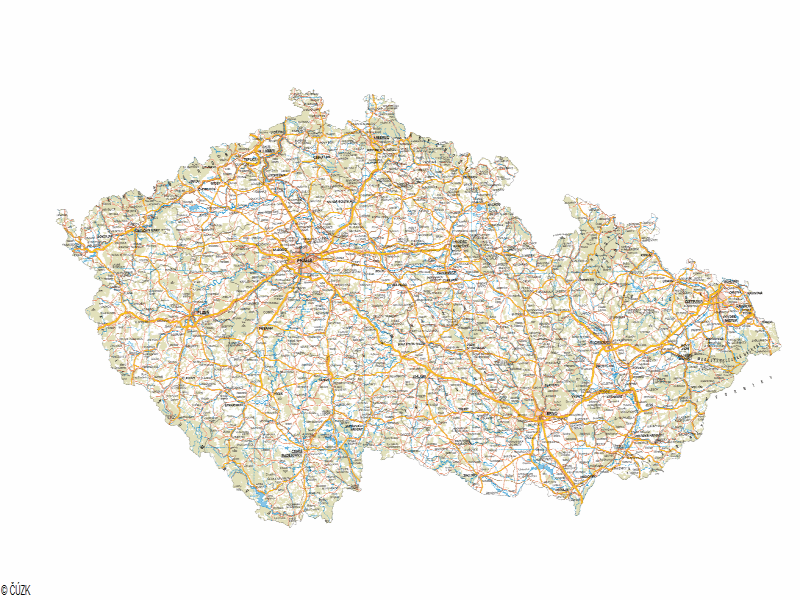
\includegraphics[scale=0.5]{figures/GetMapResponse}
\end{center}

\subsubsection{Dotaz typu GetFeatureInfo}
Poslední typ dotazu je volitelný a nazývá se GetFeatureInfo. Tento
dotaz, na rozdíl od předchozích, nemusí server podporovat.  
Dotaz slouží k~získání informací o~prvcích ve vrstvě. Pokud je
v~elementu {\tt <Layer>} uveden atribut {\tt queryable} s~hodnotou {\tt 1}, je možné na
tuto vrstvu aplikovat dotaz GetFeatureInfo.

Jako příklad pro tento typ dotazu je použit WMS server Středočeského
kraje. Jedna z~WMS služeb, které tento server poskytuje, jsou zóny
integrovaného dopravního systému dostupné na
:\url{http://mapy.kr-stredocesky.cz/ids_zony_wms}. 

Nejprve se dotazem
GetaCapabilities zjistí informace o~WMS serveru a jím poskytovaných
datech.

%\newcommand{\StredoceskygetCap}{http://mapy.kr-stredocesky.cz/ids_zony_wms?SERVICE=WMS&REQUEST=GetCapabilities}
\begin{alltt}\footnotesize
http://mapy.kr-stredocesky.cz/ids\_zony\_wms?
SERVICE=WMS\&REQUEST=GetCapabilities\&VERSION=1.3.0
\end{alltt}

Z~odpovědi je patrné, že server obsahuje pouze jednu vrstvu {\tt Zony SID},
se kterou lze dále pracovat, protože její rodičovská vrstva nemá
atribut {\tt <Name>} nutný pro dotazy GetMap a GetFeatureInfo.

Vrstva je dostupná v~jediném souřadnicovém systému. Za povšimnutí
stojí opakované uvedení projekce a stejného obdélníku
{\tt BoundingBox}, v~němž jsou poskytována data jak v~kmenové vrstvě, tak
v~jejím potomku {\tt Zony SID}. Jelikož se tyto elementy vrstvy dědí, stačilo
by je uvést pouze v~kořenové vrstvě.

Na základě informací z~dotazu GetCapabilities byl vytvořen dotaz
GetMap:

%\newcommand{\StredoceskygetMap}{http://mapy.kr-stredocesky.cz/ids_zony_wms?SERVICE=WMS&REQUEST=GetMap&VERSION=1.3.0&FORMAT=image/png&LAYERS=sid_zony&CRS=EPSG:2065&BBOX=-834258.9702,-1129697.611,-651189.0329,-968639.3882&WIDTH=1000&HEIGHT=1000}
\begin{alltt}\footnotesize
http://mapy.kr-stredocesky.cz/ids\_zony\_wms?
SERVICE=WMS\&REQUEST=GetMap\&VERSION=1.3.0\&
&LAYERS=sid_zony\&FORMAT=image/png&CRS=EPSG:2065\&
BBOX=48.093144621684,11.6163532829661,51.4980192528993,19.0628256634265\&
WIDTH=1000\&HEIGHT=1000
 \end{alltt}

A~výsledný dotaz GetFeatureInfo vypadá takto:
%\newcommand{\StredoceskyGetFeatureInfo}{http://mapy.kr-stredocesky.cz/ids_zony_wms?REQUEST=GetFeatureInfo&VERSION=1.3.0&FORMAT=image/png&LAYERS=sid_zony&CRS=EPSG:2065&BBOX=-834258.9702,-1129697.611,-651189.0329,-968639.3882&WIDTH=1000&HEIGHT=1000&INFO_FORMAT=text/html&I=695&J=720&QUERY_LAYERS=sid_zony}
\begin{alltt}\footnotesize
http://mapy.kr-stredocesky.cz/ids\_zony\_wms?
REQUEST=GetFeatureInfo\&VERSION=1.3.0\&
FORMAT=image/png\&LAYERS=sid\_zony\&CRS=EPSG:2065\&
BBOX=-834258.9702,-1129697.611,-651189.0329,-968639.3882\&WIDTH=1000\&HEIGHT=1000\&
INFO\_FORMAT=text/html\&I=695\&J=720\&QUERY\_LAYERS=sid\_zony
\end{alltt}


Jak lze vidět, tento dotaz zahrnuje parametry předchozího dotazu
GetMap a přidává další:
\begin{itemize}
  \item Parametr {\tt REQUEST} uvádí typ dotazu GetFeatureInfo.
  \item Parametr {\tt INFO\_FORMAT} popisuje v~MIME tvaru formát odpovědi na tento dotaz. WMS standard neuvádí implicitní formát, který musí server podporovat. V~tomto případě se jedná o~HTML soubor. 
  \item Parametry {\tt I} a {\tt J} lokalizují prvek, na který dotaz GetFeatureInfo směřuje. Tyto souřadnice reprezentují souřadnicový systém obrázku s~jednotkami v~pixelech a začátkem v~levém horním rohu. Souřadnice os {\tt I} a {\tt J} narůstají  
        směrem vpravo resp. dolů. Interval souřadnic je dán parametry {\tt WIDTH} a {\tt HEIGHT}, kdy {\tt I}, {\tt J} mají rozsah od 0 do {\tt WIDTH} - 1 resp. od 0 do {\tt HEIGHT} - 1. Ve verzi WMS 1.1.1. se parametry  
         {\tt I} a {\tt J} označují jako {\tt X} resp. {\tt Y}.
  \item {\tt QUERY\_LAYERS} je výčet vrstev, kterých se týká dotaz GetFeatureInfo. 
\end{itemize}

  Výsledek GetMap dotazu s~bodem o~souřadnicích {\tt I}, {\tt J}  {\tt 695} a {\tt 720}:

\begin{center}
 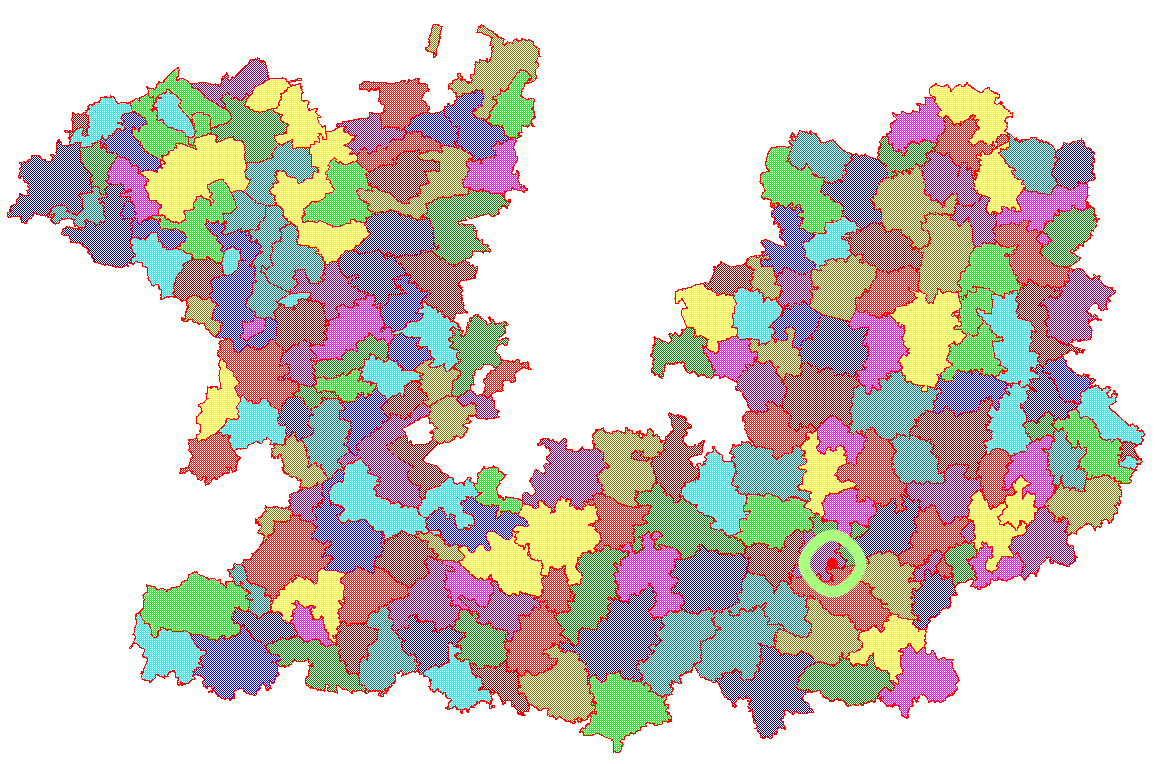
\includegraphics[scale=0.3]{figures/getfeatureinfo}
\end{center}

\newpage
A~jako odpověď server zašle HTML dokument, který se v~prohlížeči
zobrazí takto:
\begin{center}
 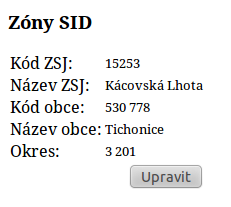
\includegraphics[scale=0.7]{figures/getfeatureinforeply}
\end{center}

Pokud je serveru položen WMS dotaz ve špatném tvaru, vrátí výjimku
implicitně ve formátu XML souboru, v~němž je blíže specifikována chyba
v~dotazu.


\newpage

\section{WMS modul pro GRASS}

Jelikož původně GRASS neměl žádné GUI, jsou jeho moduly přizpůsobeny
pro práci v~příkazové řádce. Každý modul si lze představit jako
funkci, která má definované vstupní argumenty a určené
výstupy. Nevýhodou tohoto přístupu je, že modul není schopen
s~uživatelem komunikovat za běhu. Uživatel může jeho chování ovlivnit
jen pomocí argumentů, které jsou zadány před spuštěním.

Z~tohoto důvodu implementace modulu odpovídá dotazu typu GetMap, kdy
musí být zadány parametry tohoto dotazu a modul se postará
o~stažení rastru, jeho import do GRASS a případné další úpravy.


Tento charakter modulu nebrání úplné interaktivní implementaci 
podpory WMS
do GRASS. Je ji ovšem potřeba rozdělit do dvou částí. První částí je
vytvoření modulu, který umožní pracovat s~WMS daty i uživatelům,
jenž používají pouze příkazovou řádku.  Do GUI programu je pak možné
implementovat interaktivní část.


\subsection{Analýza původního stavu}

V~GRASS GIS již existuje modul \emph{r.in.wms}\footnote{\url{http://grass.fbk.eu/grass64/manuals/html64_user/r.in.wms.html}} umožňující získání WMS dat.
Velkým problémem tohoto modulu je rozdělení jeho kódu do 8 souborů,
což jej činí velmi nepřehledným.  Tento modul byl původně napsán jako
shell skript. V~aktuální vývojářské verzi GRASS 7 byly všechny 
moduly v~shell skriptu přepsány do
jazyka Python, což také nepřispělo k~jeho zpřehlednění.

Ještě větším problémem však je, že tento modul selhává při komunikaci
s~mnoha WMS servery. Z~vlastní zkušenosti musím konstatovat, že při
používání modul spíše nefungoval než pracoval správně.

Na základě těchto faktů bylo rozhodnuto, že se WMS modul pro GRASS
vytvoří od základů znova. Případná oprava chyb ve stávajícím modulu a
reorganizace kódu by byla mnohem problematičtější a časově náročnější.

\newpage

\subsection{Stanovení cílů implementace}

Návrh struktury modulu byl realizován na základě těchto požadavků:
\begin{itemize}
  \item Modul bude plně podporovat všechny možnosti dotazu GetMap.
  \item Modul bude komunikovat se serverem prostřednictvím knihovny
    GDAL\footnote{\url{www.gdal.org/}} a také pomocí vlastní
    implementace.
  \item WMS severy mají nastaveny limity pro přenos dat, aby zabránily
    dotazům, které by je nadměrně zatížily. Tyto limity jsou dány
    formou maximálních hodnot parametrů {\tt WIDTH} a {\tt HEIGHT} dotazu GetMap.
    Modul bude umět požadavek rozdělit na více WMS dotazů a získat tak
    požadovaný rastr po částech tzv. dlaždicích, které posléze složí do
    jednoho rastru.
  \item Důležitým prvkem při práci v~systému GRASS je
    lokace. Lokace sdružuje data, která mají stejnou projekci. Její
    podmnožinou je tzv. mapset seskupující data lokace do logických
    celků.  Na začátku práce v~GRASS uživatel vybere lokaci, ve
    které chce pracovat. Následná práce je svázána s~touto lokací a
    její projekcí.
 
    Pokud by uživatel chtěl získat rastr z~WMS serveru, který
    neposkytuje data v~projekci lokace, musel by nejprve vytvořit
    lokaci v~projekci WMS dotazu a poté tyto data manuálně
    transformovat a zkopírovat do pracovní lokace.
    
    Proto bude modul schopen obdržená data automaticky transformovat
    do souřadnicového systému lokace, pokud se jejich projekce bude
    lišit.
  \item Jelikož existují další rozšíření standardu WMS, jako například
    WMTS \footnote{\url{http://www.opengeospatial.org/standards/wmts}},
    struktura modulu umožní snadnou implementaci těchto rozšíření do
    existujícího kódu.
  \item Vstupní argumenty modulu budou kompatibilní s~modulem
    \emph{r.in.wms}. Některé nevýznamné argumenty, které nemají vliv na
    funkčnost modulu, mohou být vynechány.
  \item Doplňkovou funkcí modulu bude možnost stáhnout a vypsat na
    standardní výstup obsah Capabilities souboru. Další zpracování
    tohoto výstupu bude součástí GUI.
 \end{itemize}



\subsection{Volba způsobu implementace}

V~GRASS GIS verze 7 mohou být moduly implementovány v~jazyce C nebo
Python. V~jazyce C se implementují moduly, které jsou náročné na
výpočetní výkon počítače.  Rychlost je vykoupena značně delším
vývojovým cyklem, neboť programátor je nucen se starat o~mnoho věcí,
o~které se Python postará sám.

Koncept WMS modulu byl zvolen tak, aby neprováděl žádné složité
výpočetní operace, ale aby pro tyto typy operací byly využity již
implementované funkcionality ostatních GRASS modulů nebo
knihoven. Proto byl vybrán jazyk Python.

Pro práci modulu se staženým rastrem jako je transformace a spojení
dlaždic byla zvolena knihovna GDAL, která je součástí standardní
instalace GRASS.

Tato open source knihovna umožňuje čtení, zápis a reprojekci rastrů.
Základním prvkem knihovny, který reprezentuje rastrová data je
dataset. Každý dataset reprezentuje rastrová data v~určitém formátu,
s~nimiž pracuje pomocí ovladače. Ovladač je třída, která je schopná číst
a zapisovat data v~určitém formátu.

\subsection{Volba vstupních argumentů modulu}


Vstupní argumenty budou reprezentovat jednotlivé parametry dotazu
GetMap. Počet řádků ({\tt HEIGHT}), sloupců ({\tt WIDTH}) a geografický rozsah dat
({\tt BBOX}) budou reprezentovány pomocí regionu.

Region v~GRASS je datová struktura, která definuje oblast na základě
obdélníku. Tento obdélník je dán mezními kartografickými souřadnicemi
v~každé ose a počtem řádků a sloupců. Každý region je
vztažen k~určité projekci, která je totožná s~projekcí lokace, ve
které je uložen.

Regionu určuje rozsah, na kterém bude aplikována činnost
modulů. Výjimkou jsou
moduly, které data načítají, jako je například modul \emph{r.in.gdal}\footnote{\url{http://grass.fbk.eu/grass64/manuals/html64_user/r.in.gdal.html}}. Tyto
moduly implicitně načítají data v~celém jejich rozsahu, bez ohledu na
výpočetní region.

Vstupní argumenty, které jsou nad rámec parametrů dotazu GetMap, se
týkají dlaždicování. Modul umožňuje zadání maximálního počtu řádků a
sloupců v~jednom WMS dotazu. Na základě těchto hodnot se rozdělí
stažení dat z~WMS serveru do několika dotazů a výsledný rastr je
složen z~rastrů získaných těmito dotazy.
   


\subsection{Implementace modulu}

Každý GRASS modul napsaný v~jazyce Python obsahuje funkci {\tt main}.
Tato funkce je volána při spuštění modulu. U~WMS modulu 
 funkce {\tt main} pouze vytvoří instanci tříd {\tt WMSGDALDrv} nebo {\tt WMSDrv}
v~závislosti na volbě uživatele a vše ostatní se odehrává v~rámci 
těchto instancí. Struktura modulu je popsána v~následujícím UML diagramu 
zahrnujícím nejdůležitější třídy a jejich významné metody.

\begin{center}
 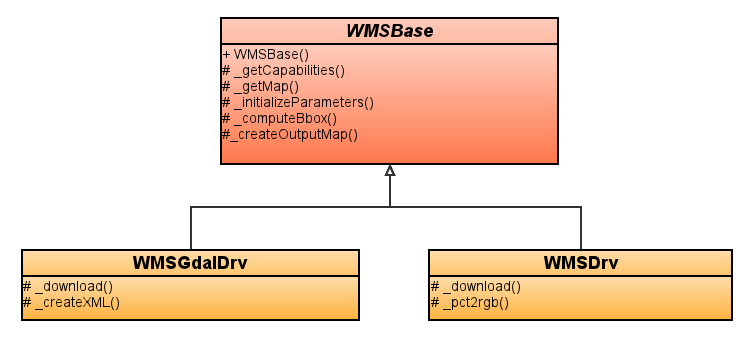
\includegraphics[scale=0.5]{figures/GRASS_UML.png}
\end{center}


Třída {\tt WMSBase} je abstraktní třída, která vykonává ty funkce, které se
netýkají komunikace s~WMS serverem, jež je implementována
v~odvozených třídách {\tt WMSGDALDrv} a {\tt WMSDrv}.

\subsubsection{Třída {\tt \bfseries WMSBase}}

Hlavními funkcemi třídy {\tt WMSBase} je výpočet parametrů pro komunikaci
s~WMS serverem, import již stažených dat do lokace a dodatečné úpravy
těchto dat pomocí modulů GRASS.

Tato třída obsahuje tyto důležité metody:  
\begin{itemize}
  \item {\tt \_GetCapabilities} - Vytvoří a pošle WMS serveru dotaz typu
    GetCapabilities, následně obdrženou odpověď vypíše na standardní
    výstup a tímto se běh modulu ukončí.
  \item {\tt \_GetMap} - Tato metoda postupně volá níže zmíněné metody
v~pořadí v~jakém jsou vedeny.
  \item {\tt \_initializeParameters} - Metoda inicializuje proměnné potřebné
    pro další běh modulu. Jde o~uložení hodnot ze slovníků vstupních
    argumentů do separátních proměnných a také získání hodnot ze
    zvoleného regionu.
  \item {\tt \_computeBbox} - Pokud se liší projekce, ve které budou data
    stažena z~WMS serveru a projekce pracovní lokace, je potřeba
    souřadnice, které vymezují region, transformovat do projekce WMS
    dotazu, aby bylo možné definovat parametr {\tt BBOX} ve správném
    souřadnicovém systému.

   Zpravidla výsledkem transformace není obdélník se stranami
   rovnoběžnými se souřadnicovými osami systému, ale obecný
   čtyřúhelník. Protože parametr {\tt BBOX} WMS dotazu GetMap musí být
   uveden v~tomto obdélníku, jsou vybrány extrémní souřadnice, které
   tvoří obdélník rovnoběžný s~osami souřadnicového systému.
  \item {\tt \_download} - Jedná se o~metodu virtuální, definovanou
v~potomcích třídy, která dotazem GetMap stáhne rastr a uloží jej do
    dočasného souboru. Zpravidla jsou rastrová data poskytována WMS
    serverem tříkanálová reprezentující RGB systém barev. Pokud jde
o~rastr s~průhlednými plochami, obsahuje ještě alfa kanál, který
    definuje průhlednost pixelů. Návratovou hodnotou metody je cesta
k~souboru s~rastrem.
  \item {\tt \_createOutputMap} - Pokud je to potřeba, tato metoda nejprve
    pomocí utility \emph{gdalwarp}\footnote{\url{http://www.gdal.org/gdalwarp.html}}
     knihovny GDAL transformuje rastr do
    projekce lokace. Transformovaný rastr je uložen do nového souboru.
    Jelikož rastr je matice o~určitých počtech sloupců a řádků, čemuž
    ale tvar transformovaného rastru zpravidla již neodpovídá, je
    potřeba mít informaci o~tom, který pixel odpovídá původnímu rastru,
    a který pixel již nereprezentuje data původního rastru. Tato
    informace je zahrnuta do alfa kanálu. Pixely, které do původního
    rastru nepatří, mají hodnotu v~alfa kanálu plně průhledného pixelu.
    Pokud transformovaný rastr neobsahuje alfa kanál, utilita
    \emph{gdalwarp} jej vytvoří.
\end{itemize}

Posléze pomocí modulu
\emph{r.in.gdal}
importuje rastrová data do pracovní lokace. Tento modul vytvoří v~pracovní
lokaci rastrové vrstvy odpovídající jednotlivým kanálům importovaného
rastru. Tyto vrstvy jsou pomocí modulu
\emph{r.composite}\footnote{\url{http://grass.fbk.eu/gdp/html_grass64/r.composite.html}}
sloučeny do jedné barevné vrstvy.

Aby byly správně interpretovány průhledné plochy výsledné rastrové
vrstvy, vytvoří se před spuštěním modulu \emph{r.composite} z~alfa kanálu
inverzní maska. Maska se v~GRASS používá v~těch případech, kdy rozsah
dat, nad nimiž bude modul pracovat, nelze vyjádřit pomocí
regionu. Maska je v~GRASS reprezentována rastrovou vrstvou, jejíž
název je {\tt MASK}. Pixely, kde je maska definována nejsou brány při
výpočtu v~úvahu.

Při použití masky vytvoří modul \emph{r.composite} barevný rastr i
s~průhlednými pixely definovanými v~alfa kanálu.

WMS modul za svého běhu vytvoří několik dočasných souborů. Tyto dočasné
soubory jsou smazány ihned poté, co již nejsou potřeba. Pokud však
uživatel neočekávaně přeruší běh programu, může se stát, že některý
soubor nebude smazán. Aby se tomuto zabránilo, je v~destruktoru třídy,
který se volá i při neočekávaném ukončení modulu, provedeno smazání
těchto souborů, jenž nebyly odstraněny. Toto je provedeno i
s~vrstvami, které reprezentují jednotlivé kanály a maskou.

\subsubsection{Třída {\tt \bfseries WMSGDALDrv}}

Tato třída přistupuje k~datům WMS serveru prostřednictvím WMS ovladače 
knihovny GDAL. Parametry WMS dotazu jsou ovladači předány ve formě XML
souboru vytvořeném metodou {\tt \_createXML}. 
 \footnote{\url{http://www.gdal.org/frmt_wms.html}}.  Metotda 
 {\tt \_download} následně stáhne data prostřednictvím GDAL ovladače a uloží 
 je do souboru.

\subsubsection{Třída {\tt \bfseries WMSDrv}}

Tato třída komunikuje se serverem přímo, bez použití další
knihovny. Nejprve je ze vstupních parametrů vytvořen WMS dotaz typu GetMap.
Pak následuje výpočet rozměrů dlaždic v~souřadnicovém systému projekce,
rozměru dlaždic v~pixelech a jejich počet. Na základě těchto hodnot
jsou v~cyklu staženy jednotlivé dlaždice, kdy je k~WMS dotazu přidán
parametr {\tt BBOX} pro konkrétní dlaždici, tento dotaz je poslán WMS
serveru a do dočasného souboru je uložen rastr z~odpovědi na dotaz. Spojování
dlaždic do jednoho rastru je řešeno pomocí knihovny GDAL. Při prvním
průchodu cyklu se vytvoří nový dataset, kde se dlaždice postupně, tak
jak jsou stahovány, spojují.

\subsection{Zajímavé problémy a jejich řešení}

Při implementaci třídy {\tt WMSDrv} se vyskytl problém při dlaždicování.
Při stažení barevného jednokanálového rastru (např. PNG, GIF)
s~přiloženou globální tabulkou barev vznikl po spojení jednotlivých
dlaždic rastr, který tuto tabulku neobsahoval.

Protože v~tomto případě konkrétní barvy jednotlivých kanálů jsou
definovány až v~tabulce barev, není možné bez této tabulky správně
interpretovat hodnoty pixelů, které zde představují pouze odkazy na
položky tabulky. V~různých dlaždicích jsou stejné barvy definovány
jinými položkami tabulky barev a hodnota pixelů na ně odkazující se
v~nich liší.  Při spojování dlaždic knihovna GDAL nebrala tabulku barev
v~úvahu a interpretovala přímo hodnoty těchto pixelů. Výsledný rastr
se spojenými dlaždicemi vypadal například takto:

\begin{center}
 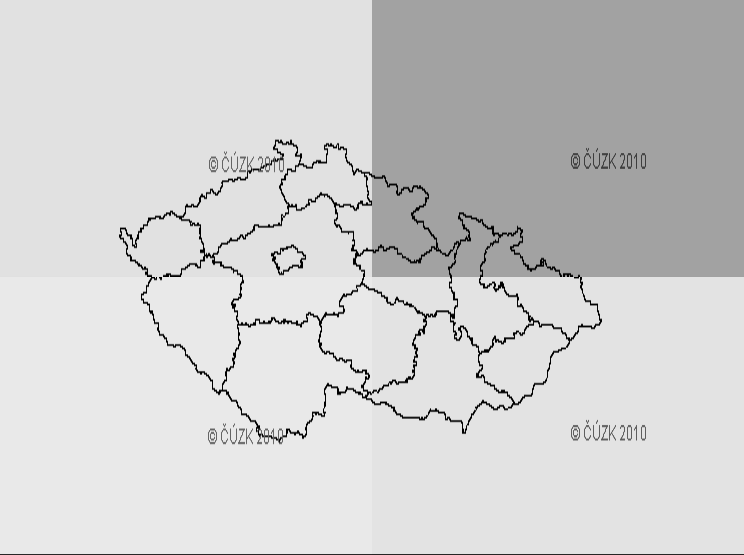
\includegraphics[scale=0.4]{figures/color_table_problem.png}
\end{center}

Tento problém byl vyřešen pomocí upraveného kódu GDAL utility
\emph{pct2rgb} \footnote{\url{www.gdal.org/pct2rgb.html}}. Tento kód obsahuje
metoda {\tt \_pct2rgb} třídy {\tt WMSGDALDrv}. Tato metoda vytvoří 4 kanálový
dataset (RGB + alfa vrstva) a do jednotlivých kanálů jsou pixel po
pixelu přiřazovány jejich hodnoty z~tabulky barev.

\subsection{Ukázka práce modulu}

Nyní je modul dostupný pod názvem \emph{r.in.wms2} v~repozitáři \emph{GRASS
AddOns} \footnote{\url{http://svn.osgeo.org/grass/grass-addons/}}.
V~tomto repozitáři jsou uloženy nové funkcionality implementované do
GRASS, které je ještě potřeba otestovat uživateli a dokončit jejich
vývoj. Až potom lze tyto funkcionality začlenit přímo do
programu.


Modul se z~repozitáře do GRASS nainstaluje pomocí tohoto příkazu:
\begin{alltt}\footnotesize
g.extension extension=r.in.wms2
\end{alltt}

\subsubsection{Vstupní argumenty}

V~GRASS GIS mají moduly dva typy vstupních argumentů. Argumenty, které
nesou binární informaci 0/1, jsou modulu předány ve formě voleb,
což řetězce uvedené za pomlčkou. Pokud je volba uvedena mezi
argumenty při spuštění modulu, nese hodnotu 1, pokud uvedena není,
je ji přiřazena hodnota 0.

\begin{table}[h]
\centering
\begin{tabular}{|c|l|}      \hline
  Volba      &    Popis				\\ \hline
   {\tt -o}        &  Data nebudou obsahovat průhlednou  vrstvu.\\ \hline
   {\tt -c}       &  Vypíše na výstup Capabilities soubor.\\ \hline
   {\tt -d }      &  Nepoužije knihovnu GDAL pro komunikaci s~WMS serverem, ale vlastní řešení. \\ \hline
\end{tabular}
\caption{Volby modulu r.in.wms2}
\label{tab:flagy}
\end{table}

Dalším typem vstupních argumentů je parametr. Parametr obsahuje jako
hodnoty textové řetězce. I~v~případě, že argument obsahuje číselnou
hodnotu, je tato hodnota uložena jako text a v~modulu musí být
převedena na číselný typ.

Volby a parametry jsou modulu předány ve slovnících {\tt flags} resp. {\tt options}. 
Tyto slovníky v~položkách obsahují název volby resp. parametru a jejich
hodnotu.

\newpage
Vstupní parametry modulu jsou:
\begin{itemize}
  \item {\tt output} - Povinný parametr. Název vrstvy vytvořené modulem
v~lokaci.
  \item {\tt mapserver} - Povinný parametr. URL adresa WMS serveru.
  \item {\tt layers} - Povinný parametr. Uvádí se ve stejném formátu jako
v~getMap parametru {\tt LAYERS}.
 \item {\tt srs} - Číslo {\tt EPSG} kódu, který definuje projekci WMS dotazu.
 \item {\tt region} - Název regionu. Pokud není uveden, je použit aktuálně
   nastavený region.
 \item {\tt wms\_version} - Verze WMS standardu, lze uvést
   {\tt 1.1.1} (implicitní), nebo {\tt 1.3.0}
 \item {\tt format} - Formát rastru WMS dotazu. Možné hodnoty jsou {\tt geotiff}
   (implicitní), {\tt tiff}, {\tt jpeg}, {\tt gif}, {\tt png}.
 \item {\tt method} - Pokud projekce rastru z~WMS dotazu a projekce lokace
   nejsou stejné, tento parametr definuje jakou metodou bude rastr
   transformován do projekce lokace. Může mít tyto hodnoty: {\tt near}
   (implicitní), {\tt bilinear}, {\tt cubic}, {\tt cubicspline}.
 \item {\tt maxrows} - Číslo, které definuje maximální počet pixelů v~řádce
   jedné dlaždice. Implicitně {\tt 400}.
 \item {\tt maxcols} - Číslo, které definuje maximální počet pixelů ve
   sloupci jedné dlaždice. Implicitně {\tt 300}.
 \item {\tt urlparams} - Zde lze uvést další parametry WMS dotazu GetMap.
                   Pouze s~volbou {\tt -o}, protože GDAL WMS ovladač toto
                   neumožňuje.
 \item {\tt styles} - Styly vrstev ve stejném formátu jako v~getMap
   parametru {\tt STYLES}.
 \item {\tt bgcolor} - Pokud je při spuštění modulu uvedena volba -o,
   budou všechny plochy,
   které by byly průhledné, vyjádřeny barvou uvedenou v~tomto
   parametru. Barva se uvádí v~hexadecimálním RGB formátu. Implicitní
   je bílá barva ({\tt 0xFFFFFF}).
\end{itemize}

\subsubsection{Příklad}
Jako příklad je použit WMS
server\footnote{\url{http://iceds.ge.ucl.ac.uk/cgi-bin/icedswms}}
poskytující družicová data. Na základě informací získaných pomocí
GetCapabilities dotazu, je možné spustit modul například s~těmito
parametry:

\begin{alltt}\footnotesize
r.in.wms2 -d mapserver=http://iceds.ge.ucl.ac.uk/cgi-bin/icedswms \\ layers=bluemarble,landsat\_1\_01 styles=default,default
output=landsat srs=4326 format=png maxcols=500 maxrows=600
\end{alltt}

Při spuštění modulu byla projekce lokace totožná s~projekci rastru
z~WMS dotazu (EPSG:{\tt 4326}). Region byl dán obdélníkem o~geografických
souřadnicích {\tt -20}° z. d., {\tt 30}° s. š., {\tt 40}° v. d., {\tt 65}° s. š. a počet
pixelů v~řádcích byl 700 a ve sloupcích 1200. Protože byl počet pixelů
v~obou dimenzích větší než parametry {\tt maxcols} a {\tt maxrows}, muselo být
stažení rastru rozděleno na stažení 4 dlaždic, které byly následně
spojeny. Data z~WMS serveru vlastní implementací, protože byla 
uvedena volba {\tt -d}.

Pro práci s~regiony je určen modul \emph{g.region}\footnote{\url{http://grass.fbk.eu/gdp/html_grass64/g.region.html}}. Pomocí tohoto modulu je
možné modifikovat parametry regionu, vytvářet regiony nové nebo zjišťovat
hodnoty parametrů regionu.


Takto vypadá stažený rastr:
\begin{center}
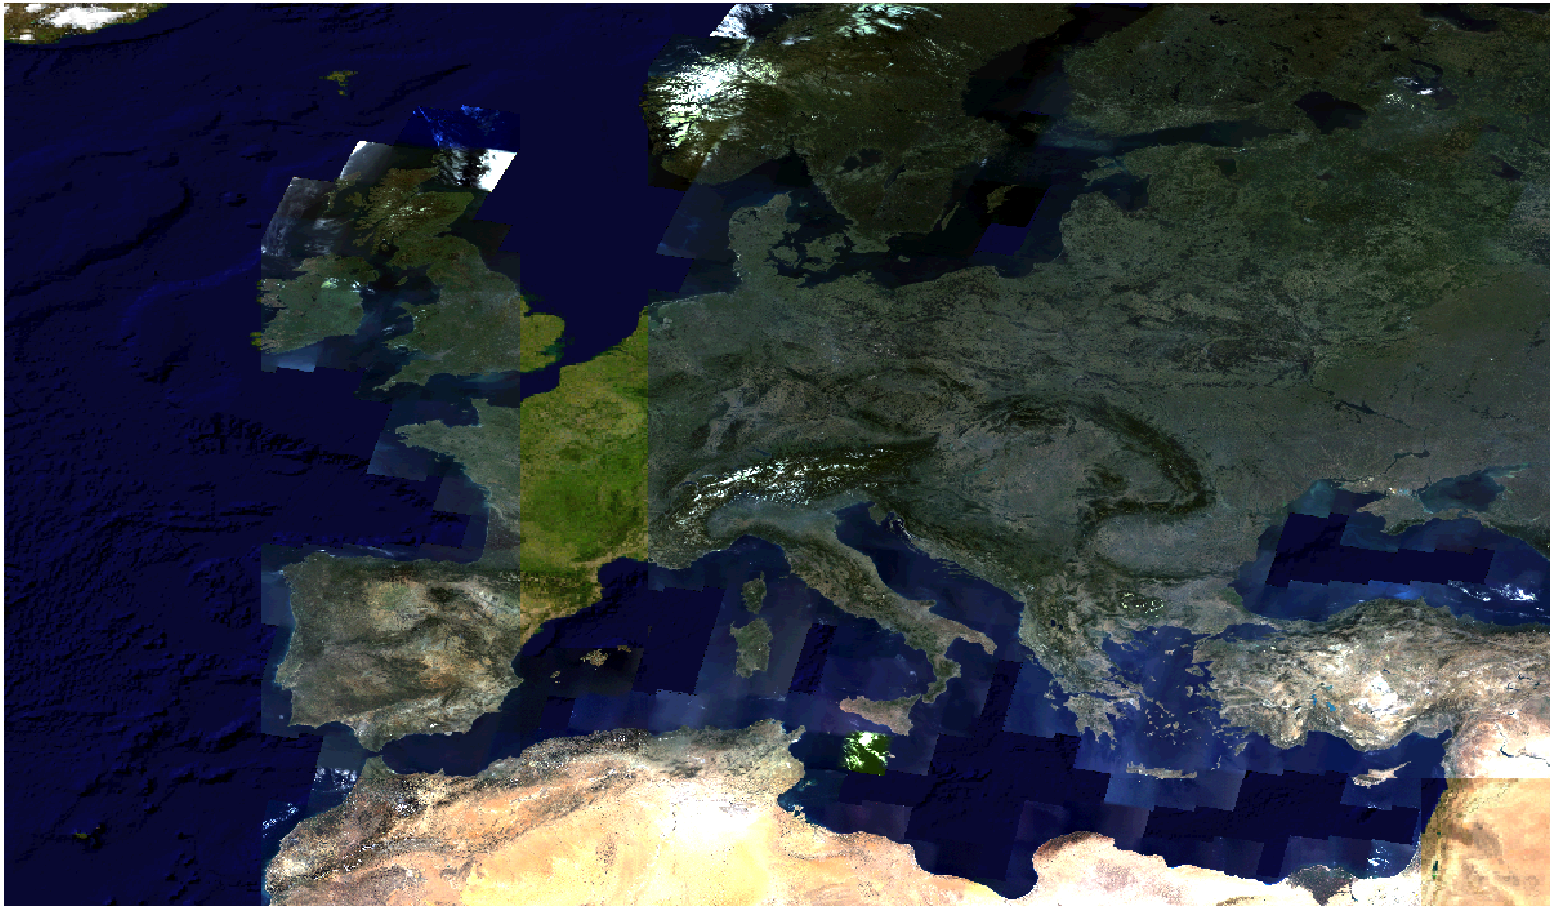
\includegraphics[scale=0.25]{figures/GRASS_WMS_obrazek.png}
\end{center}
Modul \emph{r.in.wms} v~tomto případě, jako v~mnoha ostatních, neuspěje.
Jelikož vstupní argumenty modulu \emph{r.in.wms2} jsou kompatibilní s~argumenty
modulu \emph{r.in.wms}, stačí pouze změnit název modulu  v~příkazu 
na \emph{r.in.wms} a spustit jej 
se stejnými argumenty:
\begin{alltt}\footnotesize
r.in.wms -d mapserver=http://iceds.ge.ucl.ac.uk/cgi-bin/icedswms\\ layers=bluemarble,landsat_1_01 styles=default,default output=landsat srs=432\\ format=png maxcols=500 maxrows=600
\end{alltt}
\subsection{Další vývoj}

Po otestování uživateli by se měl modul \emph{r.in.wms2} stát součástí GRASS
a nahradit modul \emph{r.in.wms}. Pokud k~tomu dojde, bude pravděpodobně
přejmenován na \emph{r.in.wms}.

Tento modul je pouze jednou částí integrace WMS do GRASS. Nyní
bude dalším krokem vytvoření interaktivního WMS řešení, které
by se uživatelskou přívětivostí přiblížilo programům
ArcGIS\footnote{\url{http://www.arcgis.com/}} nebo
QGIS\footnote{\url{http://www.qgis.org/}}. Tyto programy mají z~uživatelského
pohledu velmi dobrou podporu WMS.

Idea tohoto řešení je, že uživatel si na základě dialogu
vygenerovaného z~Capabilities souboru vybere data, která chce zobrazit
a v~GRASS GUI se přidá nová WMS vrstva. Tato vrstva bude dynamicky
získávat data, v~závislosti na aktuálním rozsahu mapového okna.

Ve vývojové verzi GRASS 7 již existuje dialogové okno, které na základě 
vložené URL adresy stáhne Capabilities soubor a z~tohoto souboru zobrazí
dostupné vrstvy.

Tento dialog funguje tak, že po zadání URL adresy se zavolá modul
\emph{r.in.wms} a ten na standardní výstup vypíše seznam vrstev
z~Capabilities souboru. Tyto vrstvy jsou pak zobrazeny v~dialogovém
okně.

Aby tento dialog umožnil uživateli využít všech možností WMS serveru,
nestačí jen vypsat seznam vrstev, ale je také potřeba zobrazit
k~výběru dostupné formáty, projekce uživatelem vybraných vrstev, styly
 a také metadata s~informacemi o~vrstvách. K~tomu nestačí jen prostý
výpis seznamu vrstev, ale je nutné pracovat s~celým obsahem
Capabilities souboru.

V~rámci bakalářské práce byly již učiněny některé kroky k~vylepšení
tohoto dialogu.

Dialog nyní využívá modul \emph{r.in.wms2}, který umožňuje vypsat celý obsah
Capabilities souboru na standardní výstup. Tento výstup je načten a
posléze zpracován do takové datové struktury, která ke každé vrstvě
umožňuje zjistit seznam elementů včetně těch děděných, což je největší
problém při zpracování Capabilities souboru. Na základě této struktury
lze v~dialogu zobrazit strom vrstev, který odráží uspořádání elementů
{\tt <Layer>} v~Capabilities souboru.

Dialog obsahuje textové pole, které bude sloužit k~informací 
o~jednotlivých vrstvách. V~aktuální podobě vypisuje pouze část informací.

Takto vypadá aktuální verze WMS dialogu v~GRASS:
\begin{center}
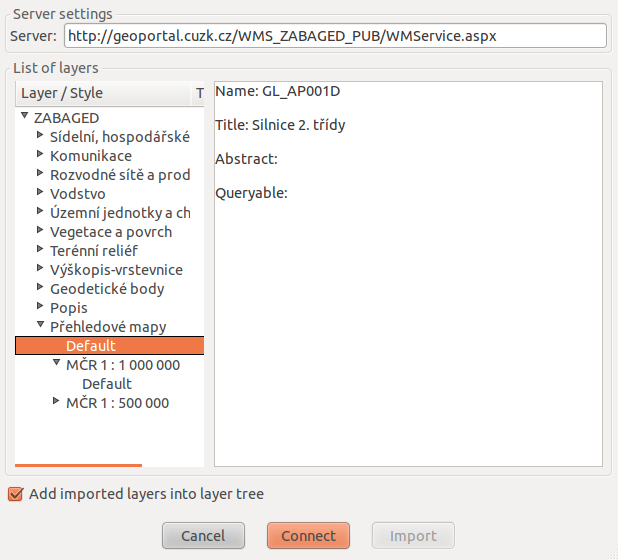
\includegraphics[scale=0.5]{figures/GRASS_dialog_soucasny_stav.png}
\end{center}


 Dalším krokem bude v~GUI vytvořit rastrovou WMS vrstvu, která, pokud
 bude zobrazena v~mapovém okně, bude zobrazovat WMS data pomocí 
 modulu  \emph{r.in.wms}. Tento
 modul bude spouštěn s~parametry, které budou zadány v~dialogovém okně
 před přidáním vrstvy. Při každém volání z~mapového okna se změní
 pouze parametr region, který bude odpovídat aktuálnímu rozsahu a
 rozlišení pixelu mapového okna.
 
Data rastru se v~mapovém okně vykreslují na základě dvou parametrů. Těmito 
parametry jsou rozsah, který je určen souřadnicemi projekce a rozměry 
pixelu. Pokud se změní rozsah i rozměr pixelu dochází k~tzv. zoomování
a je potřeba data v~celém mapovém okně vykreslit znova. 
   
Při pohybu mapového okna se mění pouze rozsah. 
Často se stává, že uživatel pohne s~oknem jen o~kousek, kdy
značná část okna je pořád v~rozsahu již stažených dat. V~tomto případě
je zde prostor pro optimalizaci, kdy by nebylo potřeba  získávat
z~WMS serveru všechna data v~rozsahu mapového okna, ale pouze ta data,
která dosud nebyla stažena. 


\newpage

\section{ WMS modul pro SAGA GIS}

Koncept modulu v~SAGA GIS je odlišný od GRASS. Moduly v~SAGA GIS
mohou i za svého běhu komunikovat s~uživatelem a reagovat na jeho 
podněty. Tyto vlastnosti lze velmi dobře využít při implementaci
 WMS.


\subsection{Analýza původního stavu}

Do aktuální verze (2.0.8) SAGA GIS byla nově začleněna experimentální
knihovna \emph{Garden - Web Service Data Access}. Tato knihovna obsahuje
modul \emph{Import a Map via Web Map Service (WMS)} umožňující získat
data z~WMS serveru.  Modul funguje tak, že po spuštění vytvoří ze
zadané URL adresy dotaz GetCapabilities a na základě odpovědi vytvoří
dialog, ve kterém si uživatel může vybrat parametry pro získání rastru
z~WMS serveru.

Toto řešení WMS modulu je uživatelsky velmi přívětivé, jelikož
 stačí pouze znát URL adresu WMS serveru a ostatní kroky 
 vedoucí k~získání dat z~WMS serveru jsou již v~režii modulu.


Jelikož se jedná o~experimentální modul v~první verzi, má určité
nedostatky. Mezi největší patří:
\begin{itemize}
\item Nezobrazí uživateli všechny možnosti, které server nabízí,
      protože špatně zpracovává Capabilities soubor. Z~tohoto 
      pohledu mezi největší chyby patří: 
\begin{itemize}
 \item Modul z~Capabilities souboru načte pouze ty vrstvy, které jsou
   přímými potomky kořenové vrstvy. Ostatní vrstvy jsou ignorovány.
 \item Nelze určit pořadí vrstev, v~jakém budou zobrazeny na výsledné
   mapě.
 \item Neumožňuje výběr stylu vrstvy .
 \item Nebere v~úvahu dědičnost ve stromu vrstev.
\end{itemize}
\item Nepodporuje dlaždicování.
\end{itemize}

\subsection{Stanovení cílů implementace}


Základní koncept modulu bude stejný jako u~modulu experimentálního. To
znamená, že modul nejprve získá Capabilites soubor z~WMS serveru,
vygeneruje pro něj nabídku a na základě zvolených hodnot pomocí dotazu
GetMap stáhne požadovaný mapový rastr a naimportuje jej do programu.

Při implementaci by měly být naplněny tyto cíle:
\begin{itemize}
\item Modul bude schopen správně zpracovat Capabilities soubor
  ve standardu 1.1.1 a 1.3.0.  Jelikož ne všechny WMS servery zcela
  naplňují WMS standardy, bude napsán tak, aby nelpěl na absolutní 
  implementaci WMS standardu serverem.
\item Nabídka parametrů umožní uživateli využití všech možností WMS
  dotazu GetMap.
\item Modul bude schopen transformovat rastr do uživatelem
  požadováného zobrazení. V~SAGA GIS neexistuje ekvivalent lokace jako
  v~GRASS. S~vrstvami lze pracovat v~libovolném zobrazení. 
  Existuje i modul, který umí transformovat rastr do jiné
  projekce. Přesto tato funkcionalita může uživateli velmi ulehčit práci,    
  protože se často stává, že WMS server neposkytuje data
v~uživatelem požadované  projekci.  
  
  Také modul umožní zadat hodnotu parametru {\tt BBOX}
v~souřadnicích požadované projekce a za běhu modulu tyto souřadnice
  transformovat do projekce WMS dotazu.
\item Umožní implementovat další rozšíření WMS standardu.
\end{itemize}


\subsection{Volba způsobu implementace}

Modul byl implementován v~jazyce C++, stejně jako ostatní moduly v~SAGA GIS. 
Byla snaha využít objektových rysů tohoto jazyka, které mohou ulehčit 
budoucí rozšiřování modulu o~podporu dalších nástaveb WMS a celkově 
pomoci vytvořit čitelnější kód.

Důležitou volbou, před vlastní implementací modulu, bylo
rozhodnutí, zda spouštět další SAGA moduly, které by
například transformovaly rastr do požadované projekce nebo
transformovaly souřadnice.

Nakonec bylo rozhodnuto tyto operace provést před importem do SAGA GIS
pomocí knihovny GDAL (reprojekce) a knihovny PROJ4 (transformace
souřadnic), jelikož spouštění ostatních modulů z~modulu není v~SAGA
GIS tak jednoduché jako v~GRASS, kde je možné modul zavolat
prostřednictvím jediné funkce. 

SAGA moduly jsou kompilovány do dynamických knihoven, které jsou po stratu 
programu načteny. Problémem je nutnost uvedení
cesty v~souborovém systému, kde se nachází knihovna zahrnující 
spouštěný modul. Knihovny jsou instalovány do určeného adresáře, avšak 
nelze vyloučit, že uživatel může tyto knihovny přesunout do jiných
 adresářů a v~tomto případě by nebylo možné modul spustit. 

Knihovna PROJ4 \footnote{\url{http://trac.osgeo.org/proj/}} je open source
projekt, který dovoluje transformovat souřadnice do různých projekcí,
které jsou součástí této knihovny. Také umožňuje definovat vlastní
projekce. Tuto knihovnu používá např. GRASS, SAGA GIS nebo GDAL.

\subsection{Moduly v~SAGA GIS}

Každý modul v~SAGA GIS je potomkem třídy {\tt CSG\_Modul}. Vstupní argumenty
modulu, které se zadávají před spuštěním, jsou uvedeny v~konstruktoru
třídy modulu.

Argumenty jsou prvky instance třídy {\tt CSG\_Parameters} {\tt Parameters}.
Metoda {\tt OnExecute} je další metoda, kterou musí každý modul
obsahovat. Tato metoda je volána při spuštění modulu.

V~SAGA GIS také existují interaktivní moduly, které jsou schopny
reagovat např. na kliky v~mapovém okně nebo na stisky kláves, jejichž
struktura se liší.


\subsection{Implementace modulu}
Modul je implementován jako přímý potomek třídy CSG\_Module. Tato
třída se nazývá {\tt CWMS\_Import} a má na starosti všechny funkce, které
jsou přímo spojeny s~programem SAGA GIS. To znamená, že tato třída 
využívá částí SAGA API. Ostatní třídy modulu jsou na SAGA API nezávislé. 
 

{\tt CWMS\_Import} vytváří dialogy na základě Capabilities souboru, který je
stažen a načten skrz členy třídy {\tt CWMS\_Base} a importuje rastr do
programu. K~těmto činnostem modul používá instance tříd definovaných
v~SAGA API. 

Jádrem modulu je metoda {\tt OnExecute}, ze které jsou volány všechny 
ostatní prvky kódu modulu.

Struktura modulu je popsána v~následujícím UML diagramu 
zahrnujícím nejdůležitější třídy a jejich významné metody a členy:

\begin{center}
 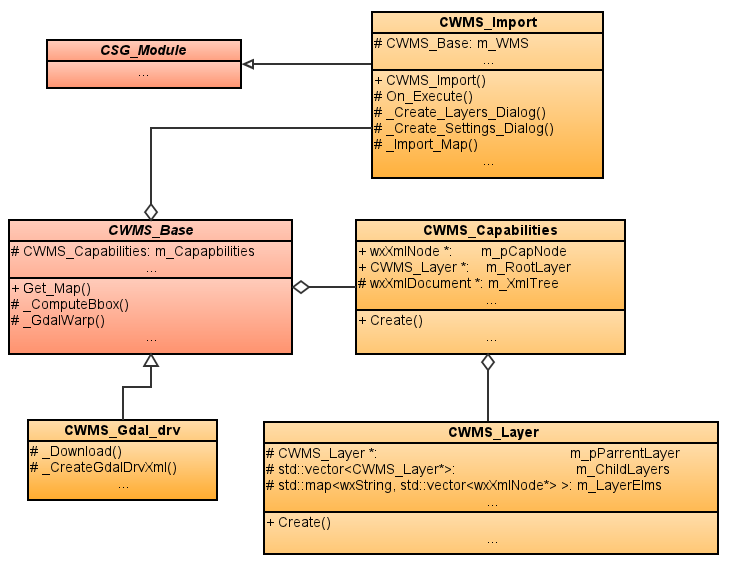
\includegraphics[scale=0.6]{figures/SAGA_UML.png}
\end{center}



\subsubsection{Třída  {\tt \bfseries CWMS\_Base}}

Tato třída nejprve pomocí instance  {\tt CWMS\_Capabilities} získá
Capabilities data z~WMS serveru. Na základě těchto dat instance
 {\tt CWMS\_Import} vygeneruje dvě nabídky, ze kterých uživatel vybere
parametry dotazu GetMap.

Potom je spuštěna metoda {\tt GetMap}, která stáhne a transformuje rastr do
požadované projekce. Tato metoda vrátí cestu k~souboru, ve kterém je
uložena již výsledná rastrová mapa určená k~načtení do programu.
Struktura a funkce této metody jsou velmi podobné WMS modulu pro
GRASS. Největším rozdílem je to, že nenačítá výslednou mapu do
programu, protože k~tomu je potřeba využít neveřejných členů třídy
{\tt CSG\_Module}, které nejsou z~této třídy dostupné. Toto by šlo obejít
deklarováním {\tt CWMS\_Base} přítelem {\tt CWMS\_Import}, což je potomek
{\tt CSG\_Module}. Tato deklarace však porušuje zapouzdřenost, jeden ze
základních principů objektově orientovaného programování. Proto je
metoda {\tt \_Import\_Map} součástí třídy {\tt CWMS\_Import}, z~níž může
přistupovat k~těmto členům.
 
Metoda {\tt \_Import\_Map} importující rastr do programu je jedinou 
částí modulu, která byla převzata z~původního modulu a nebyla
zásadně upravena.
  

Metoda {\tt Get\_Map} volá tři neveřejné metody v~tomto pořadí:
\begin{itemize}
 \item {\tt \_ComputeBbox} - Transformuje souřadnice obdélníku do
   projekce WMS dotazu.
   Transformace je provedena pomocí knihovny PROJ4, která je 
   standardně přítomna v~každé SAGA instalaci. Z~transformovaných 
   bodů jsou vybrány extrémní souřadnice, které pak definují 
   parametr {\tt BBOX} WNS dotazu.
 \item {\tt \_Download} - Tato metoda je virtuální a je pouze v~této třídě
   deklarovaná.  Návratovou hodnotou metody je cesta k~souboru
   rastru, ve kterém jsou již spojeny dlaždice z~jednotlivých WMS
   dotazů.
 \item {\tt \_GdalWarp} - Tato metoda pomocí knihovny GDAL transformuje 
   stažený rastr do výsledné projekce. Jedná se
   o~modifikovaný kód z~\url{http://www.gdal.org/warptut.html}.
\end{itemize}

\subsubsection{Třída {\tt CWMS\_Gdal\_drv}}


Členění této třídy a funkce metod jsou v~zásadě stejné jako
u~třídy {\tt WMSGDALDrv} v~GRASS modulu. Metoda {\tt \_CreateGdalDrvXml} vytvoří XML
soubor s~parametry pro GDAL WMS ovladač, který metoda {\tt \_Download}
použije pro stažení rastru z~WMS serveru.


\subsubsection{Třída {\tt CWMS\_Capabilities}}

Tato třída pomocí metody {\tt Create}, jejíž vstupním argumentem je URL 
adresa WMS serveru, vytvoří WMS dotaz GetCapabilities a následně
načte do své struktury XML soubor s~odpovědí.

K~načtení XML souboru jsou použity třídy knihovny WxWidgets \footnote{\url{http://www.wxwidgets.org/}}, která je
součástí programu SAGA. Pomocí třídy {\tt wxXmlDocument} této knihovny je
načten XML soubor a vytvořena datová struktura reprezentující strom
elementů tohoto souboru. Ekvivalentem XML elementu v~této struktuře 
je třída {\tt wxXmlNode}, která obsahuje odkaz na rodiče a na své přímé potomky.

Pokud by neexistovala dědičnost ve stromu elementů {\tt <Layer>}, bylo by
možné snadno zjistit všechny informace o~vrstvě z~jejího {\tt wxXmlNode} a
stačilo by pouze uchovat ve třídě {\tt CWMS\_Capabilities} odkaz na kořenový
element XML souboru. Protože však tato dědičnost existuje, bylo
potřeba nějakým způsobem ke každé vrstvě seskupit všechny její
elementy, včetně zděděných.
  

Proto byla vytvořena třída {\tt CWMS\_Layer}, která obsahuje ukazatel na
rodičovskou vrstvu a na její přímé potomky ve stromu. Důležitým členem
třídy je kontejner standardní knihovny C++ map s~názvem {\tt m\_LayerElms}, 
který obsahuje položky mající jako klíč název elementu, 
který je přímým potomkem nebo elementem děděným elementem {\tt <Layer>} a hodnotou tohoto 
klíče je vektor ukazatelů na objekty {\tt wxXmlNode} reprezentující elementy
s~tímto názvem.
Jelikož se jedná o~ukazatele na objekty, nejsou
ukládány duplicitní informace, ale všechny vrstvy, které dědí stejný
element odkazují na tentýž objekt.
 Například pro elementy  {\tt <Style>} je v~tomto kontejneru 
vytvořena nová položka, jejímž klíčem je text  {\tt Style} s~vektorem,
který odkazuje na všechny elementy  {\tt <Style>} prostřednictvím objektu
 {\tt wXmlNode}. 


Toto uspořádání je vytvořeno rekurzivně, kdy je strom elementů {\tt<Layer>}
procházen od kořene k~jeho listům. Po vytvoření instance {\tt CWMS\_Layer}
je zavolána její metoda {\tt Create}, která z~kontejneru {\tt m\_LayerElms}
rodičovského objektu třídy {\tt CWMS\_Layer}, který je již díky rekurzi
vytvořen, vybere ty objekty, které dědí a naplní vlastní kontejner
{\tt m\_LayerElms}. Aby kontejner obsahoval všechny přímé potomky elementu
{\tt <Layer>}, jsou potom přidány elementy, které se nedědí.

\newpage
\subsection{Ukázka práce modulu}

Pokud je modul načten do SAGA GIS, je dostupný v~knihovně modulů \emph{Web
Service Data Access} pod názvem \emph{WMS}. Po otevření modulu se objeví toto
dialogové okno:

 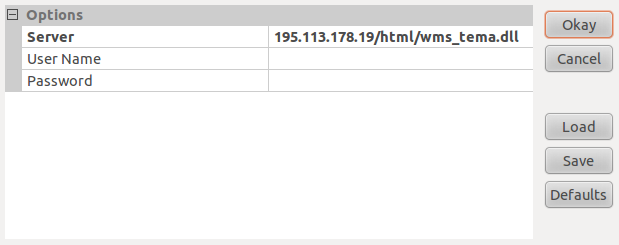
\includegraphics[scale=0.4]{figures/SAGA_okno1.png}

V~tomto případě byla zadána URL adresa WMS serveru Pardubického
kraje.  Pokud server vyžaduje uživatelské jméno a heslo, lze tyto
parametry zadat do polí {\tt User Name} resp. {\tt Password}.

Jako další dialog se zobrazí strom vrstev, které server poskytuje:

 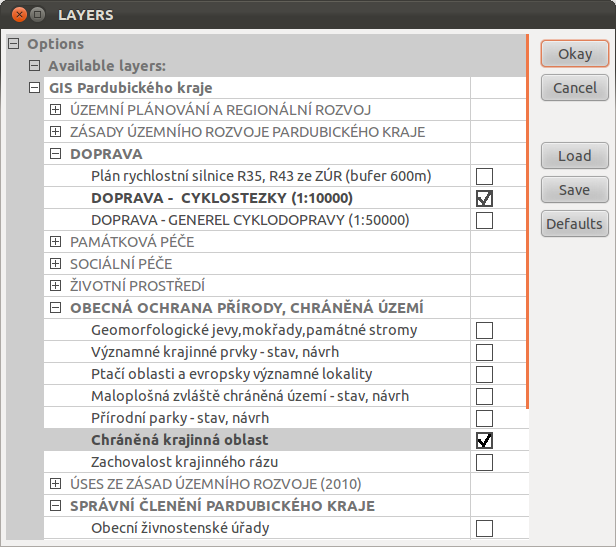
\includegraphics[scale=0.6]{figures/SAGA_okno2.png}
 
Je možné vybrat pouze ty vrstvy, které mají definován uveden element
{\tt <Title>}. Jak bylo již výše zmíněno, vrstvy které tento element
postrádají nelze použít pro dotaz typu GetMap.
 

 Posledním dialogem generovaným modulem je nastavení parametrů WMS
 dotazu.  Pro tento příklad, kdy byly vybrány vrstvy {\tt Obce s~rozšířenou
 působností}, {\tt Hranice obcí}, {\tt DOPRAVA - CYKLOSTEZKY (1:0000)} a {\tt Chráněná
 krajinná oblast vypadá takto}:
 
  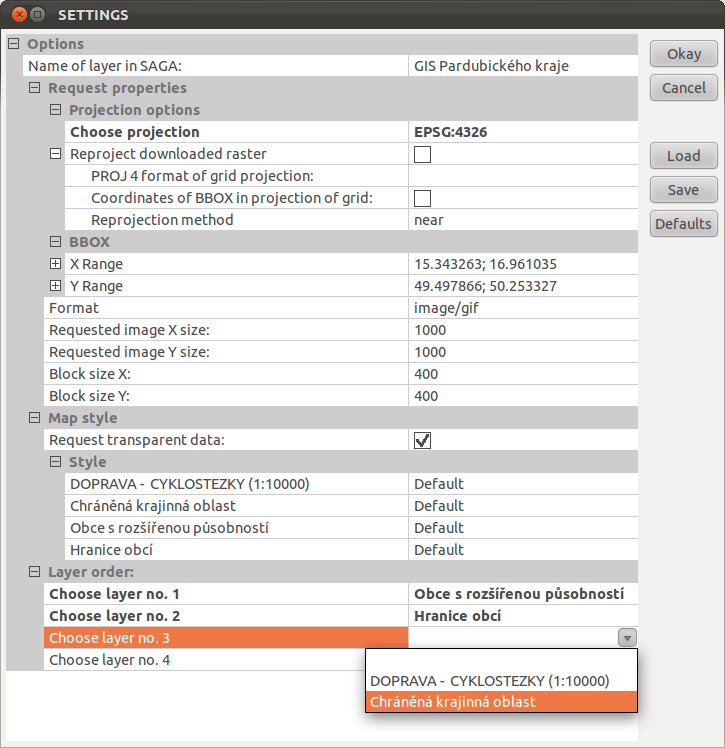
\includegraphics[scale=0.6]{figures/SAGA_okno3.png}

\newpage
Dialog obsahuje tyto položky:

\begin{itemize}
\item {\tt Name of layer in SAGA} - Představuje název vrstvy se 
      staženými rastrem v~SAGA.
\item {\tt Choose projection} - Tato nabídka obsahuje seznam všech společných
  projekcí, ve kterých jsou dostupné vybrané WMS vrstvy. Pokud uživatel
  změní vybranou projekci, jsou automaticky změněny hodnoty v~oddíle
  {\tt BBOX}, na  hodnoty pro tuto projekci z~elementu {\tt <BoundingBox>}. 
  Toto slouží k~usnadnění orientace uživatele, v~jakém rozsahu 
  jsou data poskytována.
\item Pokud uživatel chce rastr stažený z~WMS serveru transformovat 
  do jiné projekce,
  definuje tuto projekci v~parametru {\tt PROJ4 format of grid projection}. 
  Pokud má  být rastr transformován, musí také být zatržena volba
  {\tt Reproject  downloaded raster}. Jestliže jsou zadány souřadnice {\tt BBOX}
  v~projekci, do které rastr bude transformován, je potřeba
  zatrhnout volbu  {\tt Coordinates of BBOX in projection of grid}.
\item Po oddíle {\tt BBOX} jsou definovány rozměry staženého rastru
v~pixelech ({\tt Requested image X/Y size})a počet pixelů v~řádcích a
  sloupcích jedné dlaždice ({\tt Block size X/Y}).
\item V~oddíle {\tt Map Style} volba {\tt Request transparent data} udává, zda
  mají být požadovány data s~průhlednou vrstvou.  V~pododdíle {\tt Style}
  jsou zobrazeny nabídky se všemi dostupnými styly jednotlivých
  vrstev.
\item V~posledním oddíle je možné určit pořadí vrstev, v~jakém budou
  budou vykresleny ve výsledné mapě. Aby si uživatel nemusel
  pamatovat, které vrstvy již vybral ve výše uvedených nabídkách, jsou
  již vybrané vrstvy z~těchto nabídek odstraněny.  Výběr pořadí vrstev
  by bylo lepší implementovat jako seznam položek, které by šlo
  přesouvat. Avšak SAGA API neumožňuje vytvořit takovýto prvek
v~dialogu modulu.
\end{itemize}


WMS server v~tomto příkladě nepodporuje standard zcela
správně. Problémem je, že vrstvy řadí v~opačném pořadí, takže ta vrstva,
která je vybraná jako první (Obce s~rozšířenou působností), bude
překryta ostatními vrstvami. Pokud by se WMS server choval správně,
měla by být zobrazena nad všemi vrstvami.


Následně na základě zvolených parametrů modul stáhne data z~WMS
serveru a importuje je do SAGA GIS. V~tomto případě stažená data
vypadají takto:

 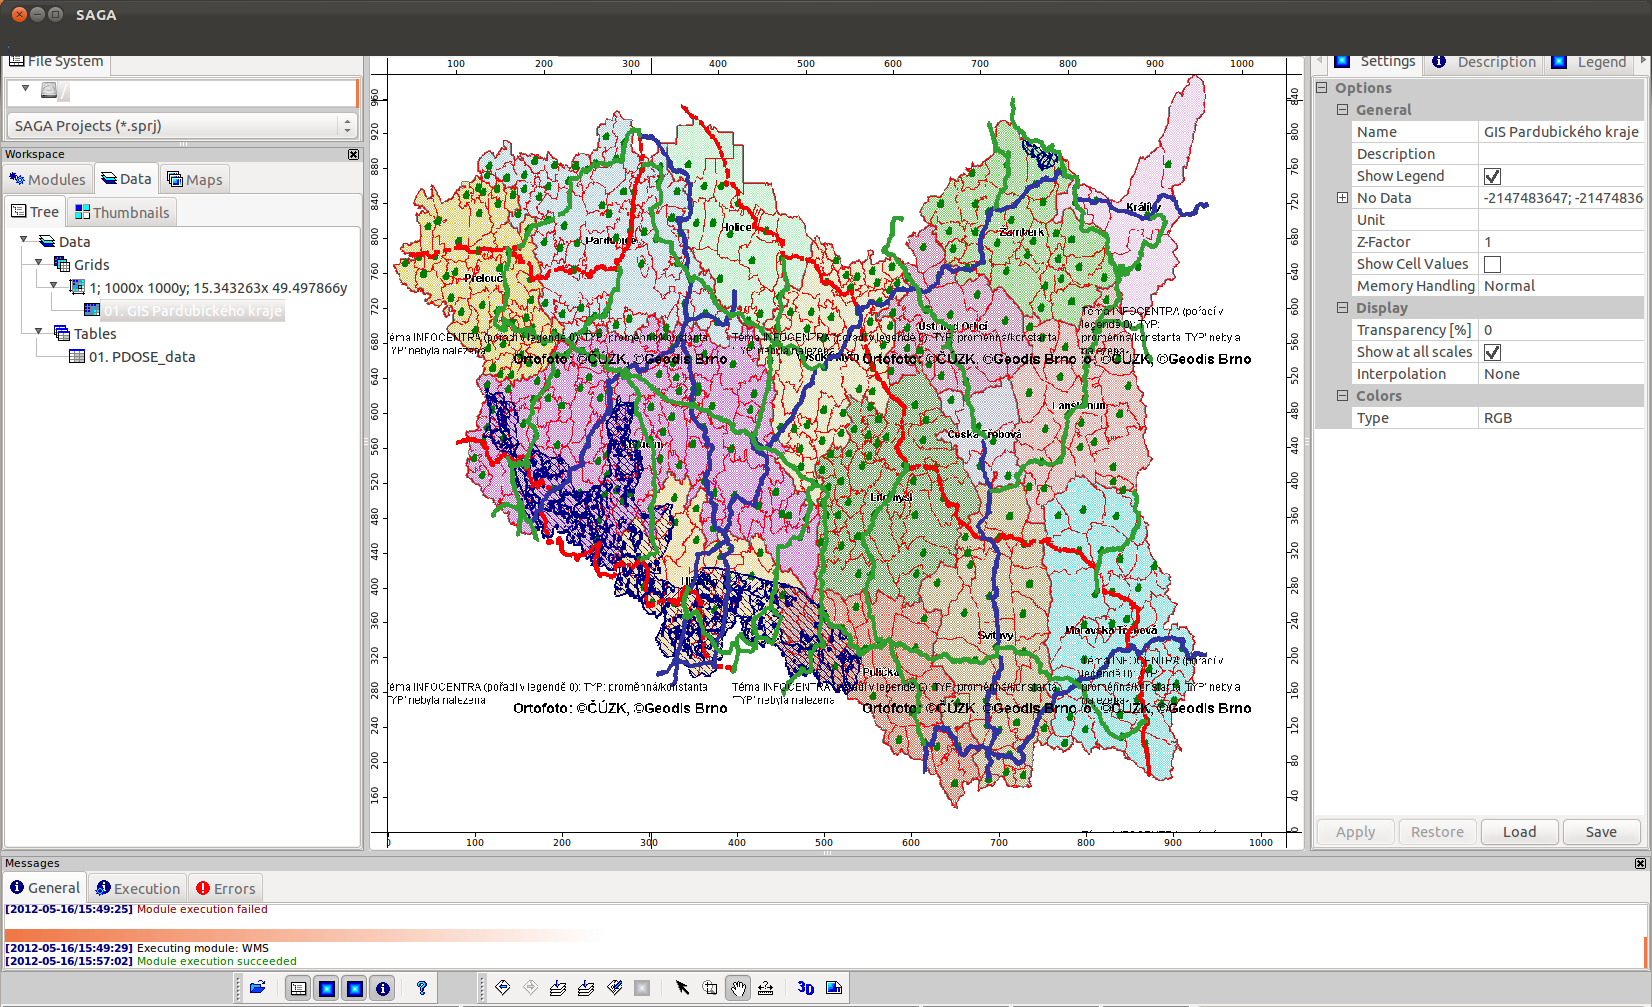
\includegraphics[scale=0.25]{figures/SAGA_okno4.png}
 
 

Původní modul na tomto příkladě selže, protože nenabídne uživateli 
žádné vrstvy, jelikož v~úvahu bere pouze vrstvy, které jsou 
přímým potomkem kořenové vrstvy (např. {\tt DOPRAVA}) a v~tomto příkladě 
jsou všechny tyto vrstvy 
bez elementu {\tt <Title>}, čili nepoužitelné pro dotaz GetMap. 
Dialog, který modul vygeneruje v~tomto příkladě vypadá takto:

 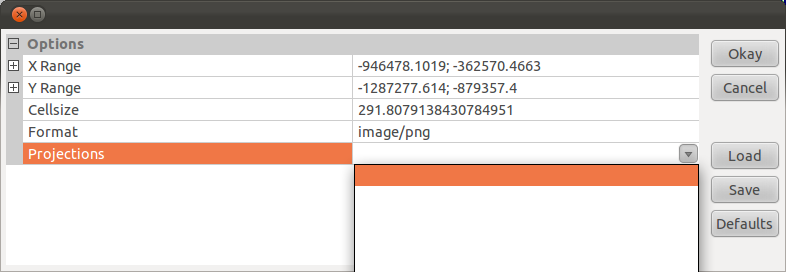
\includegraphics[scale=0.5]{figures/SAGA_puvodni_modul.png}
 
Protože modul generuje pouze jeden dialog, měl by obsahovat i 
nabídku vrstev, které v~tomto případě nenačte. Jak je vidět,
dalším problémem je špatné načtení informací o~projekci, kdy 
položky výběru jsou prázdné. 
Toto není jediný problém  spojený s~projekcemi. Protože modul načítá 
projekce rovněž z~kořenového elementu, není schopen nabídnout, ty projekce 
které jsou uvedeny u~vrstev níže ve stromu. 

\subsection{Další vývoj}

Nejdůležitějším krokem, který by se měl udát v~blízké době, bude
zveřejnění modulu komunitě uživatelů SAGA, aby bylo
možné modul řádně otestovat a upravit jej podle připomínek
uživatelů. Způsob zveřejnění bude muset být ještě dohodnut s~vývojáři
SAGA.

Do modulu by měla být přidána nová třída {\tt CWMS\_Drv}, která bude přímo
implementovat komunikaci s~WMS serverem. Princip této implementace
bude velmi podobný třídě {\tt WMSDrv} v~modulu GRASS. Neměl by být problém
začlenit tuto třídu do stávajícího kódu, protože stávající struktura
modulu je již k~tomu přizpůsobena.

Modul by měl běžet ve vlastním vlákně, protože pří stahování dat se
program SAGA odmlčí. Tento stav je velmi nepříjemný pokud
stažení dat trvá delší dobu. 

Dalším krokem by bylo provázání modulu s~mapovým oknem, kdy by
docházelo k~dynamickému zobrazování WMS dat v~mapovém okně na základě 
jeho aktuálního rozsahu.

K~tomuto nelze využít stávajících možností interaktivních modulů,
které mohou reagovat jen na akce vyvolané myší nebo klávesnicí.


\newpage 
\section{Závěr}

V~rámci této bakalářské práce byla vylepšena podpora WMS v~programech 
GRASS a SAGA GIS. 

V~programu GRASS byl vytvořen WMS modul, který odstraňuje problémy 
původního WMS modulu a byl navržen tak, aby byl lehce
rozšiřitelný o~podporu dalších nadstaveb WMS standardu, čímž by 
uživatelům GRASS umožnil přístup k~zdrojům dat, které jim nyní zůstávají 
do velké míry zapovězeny. Při implementaci byly naplněny všechny 
stanovené cíle. 

Také byly učiněny některé kroky v~rámci integrace  podpory WMS 
do GRASS GUI, které by měly v~budoucnu vést ke srovnatelné práci s~WMS daty
v~GRASS jako v~programech ArcGIS nebo QGIS, které jsou v~tomto špičkou 
mezi GIS aplikacemi.

V~SAGA GIS byl experimentální WMS modul, 
který má velké nedostatky, přepracován
 a jeho funkcionalita rozšířena do takového stavu, že nyní je možné 
 jej považovat za plnohodnotný WMS modul. Rovněž u~tohoto modulu byly při implementaci naplněny všechny stanovené cíle. 

Velmi zajímavou zkušeností byla práce na dvou
různých open source projektech. Co se týče projektu SAGA GIS, je zde velmi
znát, že jeho komunita je mnohem menší než komunita kolem GRASS. 
To se zejména projevuje na téměř neexistující dokumentaci pro vývojáře,
a proto je potřeba většinu informací vypátrat přímo ve zdrojovém kódu.

Další velkou zkušeností byl vývoj v~podstatě velmi podobných
funkcionalit řešící stejný problém ve dvou odlišných programovacích
jazycích Python a C++.  Díky tomu jsem měl možnost si prakticky potvrdit
známý fakt, že C++ je sice velmi silný nástroj a efektivní programovací 
jazyk, jehož odvrácenou stranou ve srovnání s~jazykem Python je mnohem 
delší a pracnější vývoj.

\newpage
\necislovana{Seznam použitých zkratek}

\begin{tabular}{ll}
\textbf{API}& Application Programming Interface\\
\textbf{CGM}& Computer Graphics Metafile\\
\textbf{EPSG}& European Petroleum Survey Group\\
\textbf{GDAL}& Geospatial Data Abstraction Library\\
\textbf{GIS}& Geographic Information System (Geografický informační systém)\\
\textbf{GPL}& General Public License\\
\textbf{GRASS}& Geographical Resources Analysis Support System\\
\textbf{GUI}& Graphical User Interface (Grafické uživatelské rozhraní)\\
\textbf{HTTP}& Hypertext Transfer Protocol\\
\textbf{JPEG}& Joint Photographic Experts Group\\
\textbf{MIME}&  Multipurpose Internet Mail Extensions\\
\textbf{PNG}& Portable Network Graphics\\
\textbf{QGIS}& Quantum GIS\\
\textbf{OGC}& Open Geospatial Consortium\\
\textbf{SAGA}& System for Automated Geoscientific Analyses\\
\textbf{SVG}& Scalable Vector Graphics\\
\textbf{TIFF}& Tag Image File Format\\
\textbf{UML}& Unified Modeling Language\\
\textbf{URL}& Uniform Resource Locator\\
\textbf{WMS}& Web Map Service\\
\textbf{WMTS}&   Web Map Tile Service\\
\textbf{XML}& Extensible Markup Language\\
\end{tabular}

\newpage
\renewcommand\baselinestretch{1.2}
\selectfont
\renewcommand{\refname}{Použité zdroje}
\phantomsection
\addcontentsline{toc}{section}{\refname}

\begin{thebibliography}{99}
\label{literatura}


\bibitem{WMS 1.3.0.}
Open Geospatial Consortium
\textit{Web Map Service Implementation Specification - Version 1.3.0"} [online]. 2004  [cit. 2012-02-22].
URL:\textless\url{http://portal.opengeospatial.org/files/?artifact_id=14416}\textgreater


\bibitem{WMS 1.1.0.}
Open Geospatial Consortium
\textit{Web Map Service Implementation Specification - Version 1.1.0"} [online]. 2002  [cit. 2012-02-22].
URL:\textless\url{http://portal.opengeospatial.org/files/?artifact_id=1081&version=1&format=pdf}\textgreater


\bibitem{grass_gis}
NETELER, Markus; MITASOVA, Helena. \textit{Open Source GIS:
A~GRASS GIS Approach}. 3rd Ed. New York: Springer, 2008. 406 s. URL:
\textless\url{http://www.grassbook.org}\textgreater. ISBN 978-0-387-35767-6.

\bibitem{wxPythonInAction}
RAPPIN, Noel; DUNN, Robin. \emph{WxPython in Action}. Greenwich, USA: Manning
Publications Co., 2006. 552 s. ISBN 1-932394-62-1.


\bibitem{sagaapi}
SAGA User Group Association. \textit{SAGA API} [online].
2011 [cit. 2012-03-22].
URL: \textless\url{http://www.saga-gis.org/saga_api_doc/html/index.html}\textgreater

\bibitem{script}
GRASS Development Team. \textit{GRASS 7 Programmer's Manual} [online].
2012 [cit. 2012-03-02].
URL: \textless\url{http://www.saga-gis.org/saga_api_doc/html/index.html
}\textgreater

\bibitem{trac}
\textit{GRASS GIS Tracker and Wiki} [online]. 2012 [cit. 2012-03-01].
URL: \textless\url{http://trac.osgeo.org/grass}\textgreater

\bibitem{gepro}
GEPRO spol s.r.o. \textit{WMS služby v~ČR} [online].
2011 [cit. 2012-02-19].
URL: \textless\url{http://www.gepro.cz/geodezie-a-projektovani/tipy-a-triky/wms/wms-sluzby-v-cr/}\textgreater

\bibitem{skylab}
SKYLAB Mobilesystems Ltd. \textit{OGC WMS Server List} [online].
2009 [cit. 2012-02-19].
URL: \textless\url{http://www.skylab-mobilesystems.com/en/wms_serverlist.html}\textgreater

% \subsection*{Webové odkazy}


\end{thebibliography}

\end{document}
